\documentclass{textreportclass}  % 这里引用类文件

\begin{document}
	% 页面风格
	\thispagestyle{empty}%使封面没有页眉页脚
	\pagestyle{bianyi}
	% 首页 ,插入封面
	\pagestyle{bianyi} % 这里在类文件已经定义了页面风格,在此引用
% {\songti\zihao{5}编号:123345,2346}
 
 
 
 
 
\vspace{2cm}
  \begin{figure}[h]
 	\centering
 	
\includegraphics[scale=1]{Fig/logo.pdf}
 %	\caption{锥形光线溢出图}
 \end{figure}
 \vspace{1cm}
 
\begin{center}
	\textbf{\bfheiti \zihao{-1}《单片机原理》实训报告}
\end{center}
 

 
\vspace{6cm}
\begin{table}[h]
	\centering
	\begin{large}
		\begin{tabular}{p{2cm} p{7cm}<{\centering}}
			\textbf{\bfsongti 课~~\quad~~题: }&  \textbf{\bfsongti 基于51单片机的多功能显示器}     \\ \cline{2-2}
			                     %             & \textbf{\bfsongti 及无敌无敌武打鸡血设计} \\ \cline{2-2}
			\textbf{\bfsongti 学~~\quad~~院:}  & \textbf{\bfsongti 数计学院(软件服务外包)} \\ \cline{2-2}
			\textbf{\bfsongti 专业班级:}  & \textbf{\bfsongti 22计外1班} \\ \cline{2-2}
			\textbf{\bfsongti 队~~\quad~员1:} & \textbf{\bfsongti 尹仁标}  \\ \cline{2-2}
			\textbf{\bfsongti 学~~\quad~号1:}& \textbf{\bfsongti 22050555111}\\ \cline{2-2}
			\textbf{\bfsongti 队~~\quad~员2:} & \textbf{\bfsongti 华文超}  \\ \cline{2-2}
			\textbf{\bfsongti 学~~\quad~号2:}& \textbf{\bfsongti 22050555134}\\ \cline{2-2}
			\textbf{\bfsongti 指导教师:   }  & \textbf{\bfsongti 杨翌虢~高级工程师} \\ \cline{2-2}
		\end{tabular}
	\end{large}		
\end{table}
 
\vspace{2cm}
 
\begin{center}
	\textbf{\bfsongti\zihao{4}\today}  % 这里日期根据生成pdf日期更新
\end{center}

\begin{center}
 	\textbf{\bfsongti \zihao{4}安博教育集团华东实训基地}
\end{center}
\newpage  
	% 正文加粗\textbf{\bfsongti 正文}
	
\newpage
\setcounter{page}{1}	
\pagestyle{bianyi}

	
\section{项目设计背景和应用场景}             %一
	
	
	
	
	\subsection{设计背景}					%1.1
	在信息技术迅猛发展的今天,微电子技术作为推动现代科技发展的关键力量,正以其前所未有的速度改变着我们的生活和工作方式。单片机,作为微电子技术领域的一个重要分支,已经成为智能设备设计和开发中的核心组件。它们之所以受到市场的广泛青睐,不仅因为体积的小巧和成本的低廉,更得益于其强大的处理能力和灵活的编程特性。这些优势使得单片机能够适应各种复杂的应用环境,满足不同用户的需求。
	随着科技的不断进步,人们对电子产品的期望也在不断提高。用户不仅希望产品具备基本的功能,更期待它们能够提供更加丰富、个性化的使用体验。正是在这样的市场需求驱动下,设计一款集成了多种功能的显示器的想法应运而生。这款显示器的设计初衷是创造出一个能够满足现代用户对智能化、个性化需求的产品。它不仅提供时间显示,还集成了闹钟、秒表、温度监测等实用功能,以及滚动特效,以增强信息展示的生动性和趣味性。通过这些功能的整合,显示器不仅能提升用户的日常生活质量,也能为专业工作环境带来便利。
	
	
	\subsection{应用场景}					%1.2
	多功能显示器的应用场景广泛,它能够轻松融入家庭、办公室、实验室等多种环境,为用户提供定制化的功能服务。在家庭环境中,这款显示器可以作为智能家居系统的一部分,与家中的其他智能设备如灯光、温度控制等协同工作,实现家庭环境的智能管理。用户可以通过它来设置闹钟,管理日常作息;通过温度显示功能,实时监控室内温度,保持舒适的居住环境。在办公室环境中,这款显示器的时间管理和秒表计时功能可以提高工作效率。员工可以利用它来安排会议、记录工作进度,同时,环境温度的实时监测可以帮助维持一个健康舒适的工作环境。此外,滚动特效的加入,可以让办公室的显示屏更加引人注目,用于展示重要信息或通知。在实验室等专业环境中,多功能显示器的秒表和温度显示功能对于科研人员来说尤为宝贵。它们可以辅助进行精确的实验操作和数据记录,确保实验的准确性。同时,滚动特效可以用于展示实验过程中的关键数据或安全提示,提高实验室工作的安全性和效率。随着社会对电子产品多功能性需求的不断增长,这款多功能显示器凭借其高度集成化和个性化的特点,有望成为市场上的新宠。它不仅满足了现代用户对智能设备多功能性的追求,更以其创新性和实用性,引领了智能显示设备发展的新趋势。
	
\section{项目介绍}				 			%二
	\subsection{51单片机介绍}			   %2.1
	51单片机是对兼容英特尔8051指令系统的单片机的统称。这种单片机由于其指令系统、内部结构相对简单,被广泛应用于家用电器、汽车电子、工业测控、通信设备等领域。51单片机因其易于编程、成本低廉、应用灵活而受到市场的青睐,也常被用于教育和培训中,作为学习微控制器原理和应用的入门平台。AT89C51是一款由Atmel公司生产的8位微控制器,它基于8051微控制器架构的单片机,80C52则是其增强版,是本项目的核心。
	\begin{figure}[htbp]
		\centering
		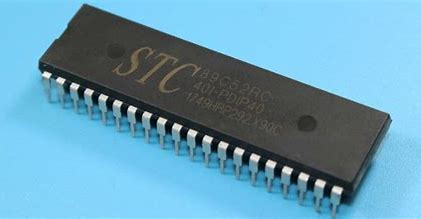
\includegraphics[scale=0.4]{Fig/AT89C51.JPG}
		\caption{51单片机CPU}\label{Fig.1}
	\end{figure}
	
	\begin{figure}[htbp]
		\centering
		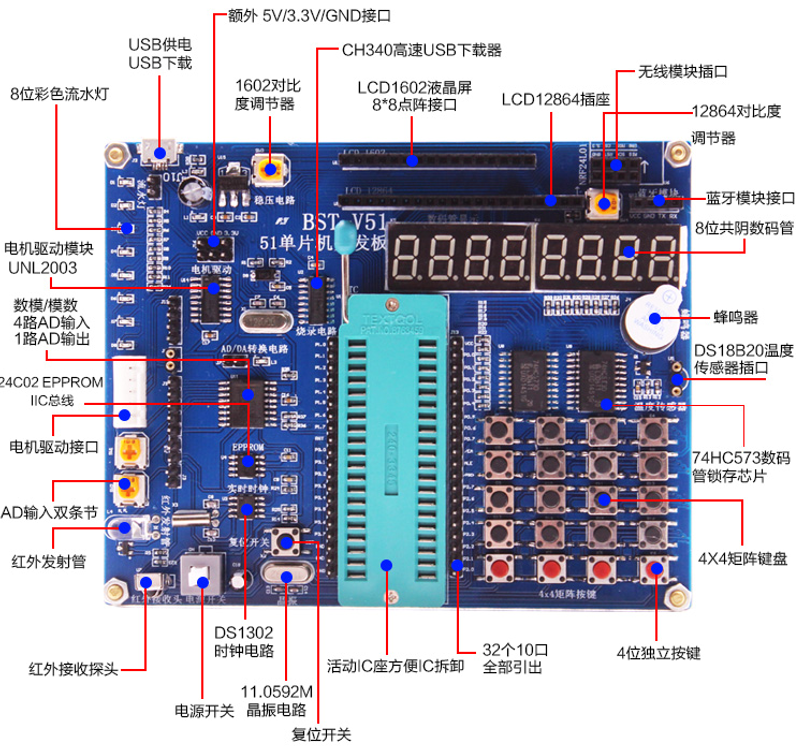
\includegraphics[scale=0.3]{Fig/51单片机主板.png}
		\caption{51单片机主板}\label{Fig.2}
	\end{figure}
	
	
	
	\subsection{项目工具和平台}			   %2.2
	项目设计方法采用结构化设计方法,使代码简洁美观。
	
	资料来源:
	\begin{itemize}
		\item Google、GitHub、Gitee、bilibili、CSDN
	\end{itemize}
	
	使用工具:
	\begin{itemize}    
		\item Keil\_5、Proteus、PZ-lsp、Visio、Visual Studio、WPS
	\end{itemize}
	
	开发语言和开发环境:
	\begin{itemize}
		\item C语言
		\item Visual Studio代码编写
		\item Keil\_5代码编译
		\item Proteus仿真图绘制
	\end{itemize}
	
	\subsection{项目组成}			       %2.3
	\begin{itemize}
		\item 多功能电子表
		\item 16x16点阵移动特效显示装置
	\end{itemize}
	\begin{figure}[htbp]
		\centering
		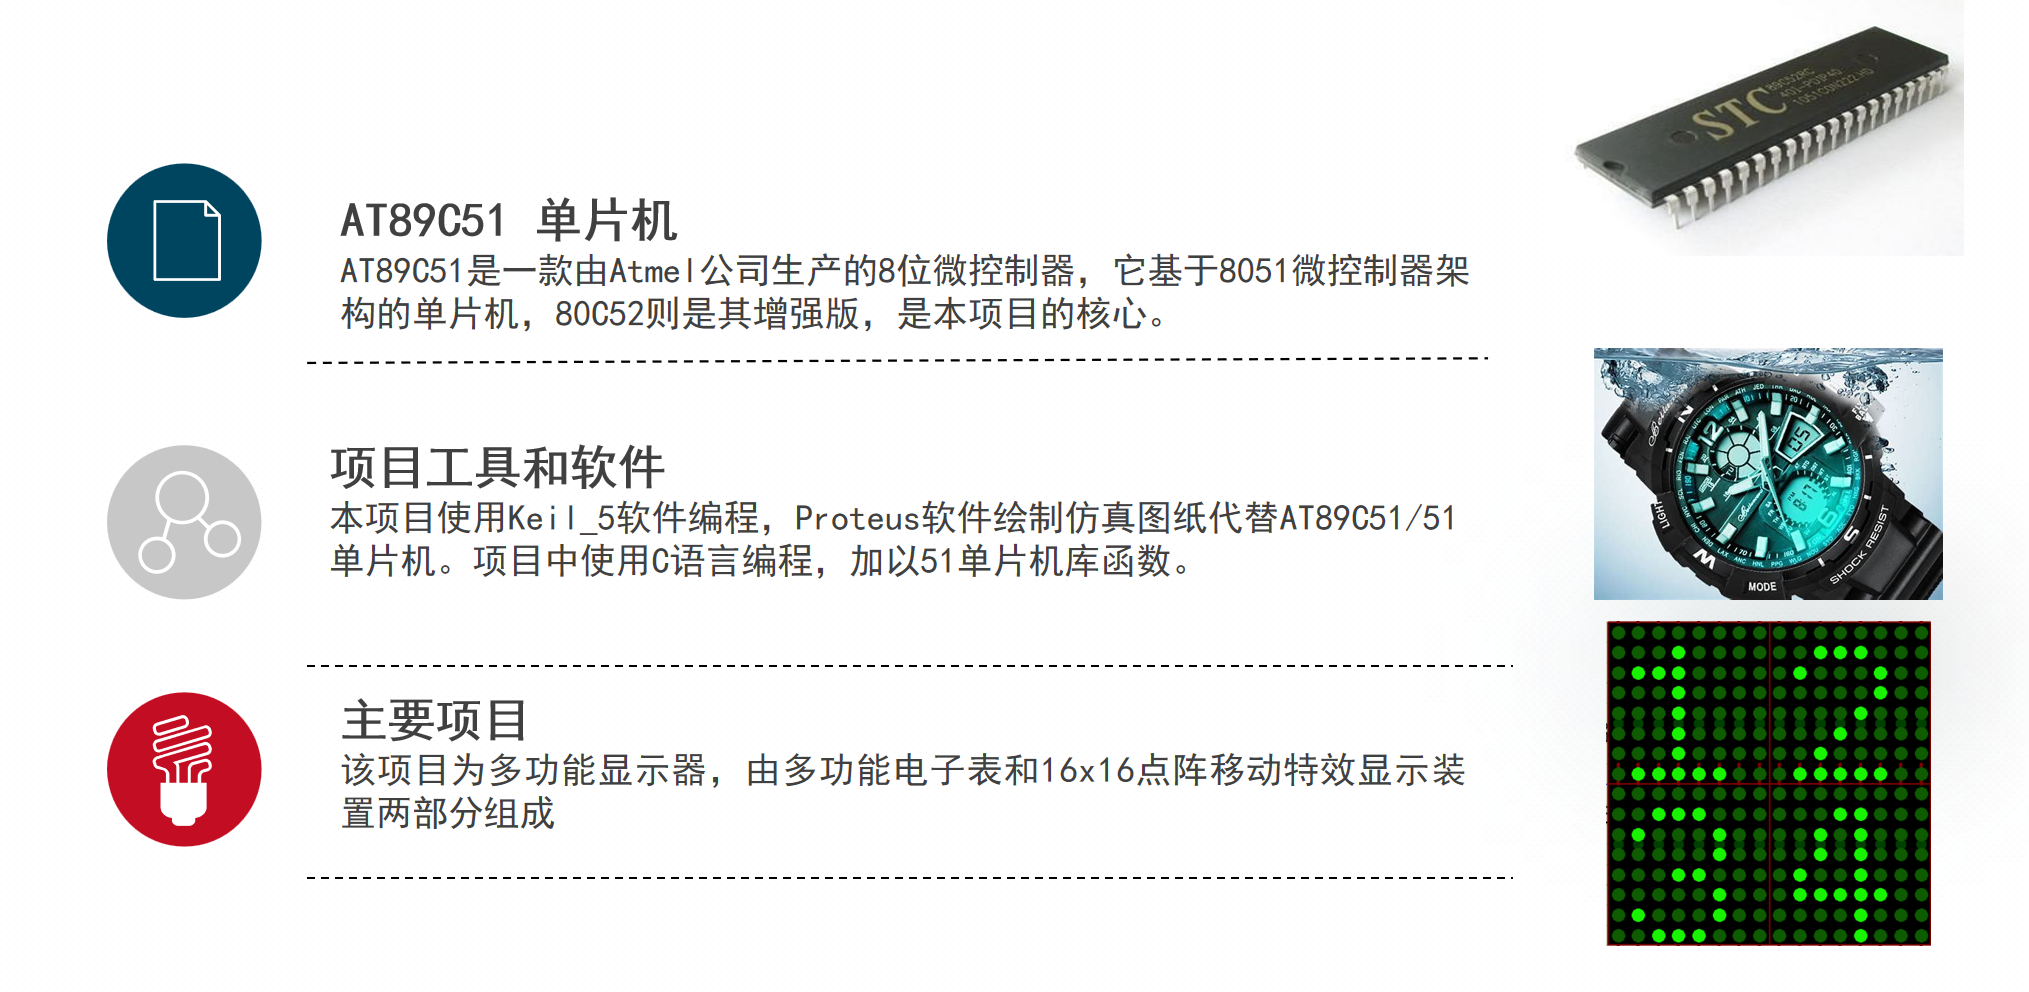
\includegraphics[scale=0.4]{Fig/简介.PNG}
		\caption{多功能显示器组成}\label{Fig.5}
	\end{figure}
	
	
\section{项目设计}				 			%三
	
	\subsection{51单片机开发板原理图}		%3.1
	51单片机开发板原理图展示了51单片机开发板电路连接和元件之间相互关系的图表。开发板通常包括单片机本身以及与之连接的各种外围设备和接口。
	
	\begin{figure}[htbp]
		\centering
		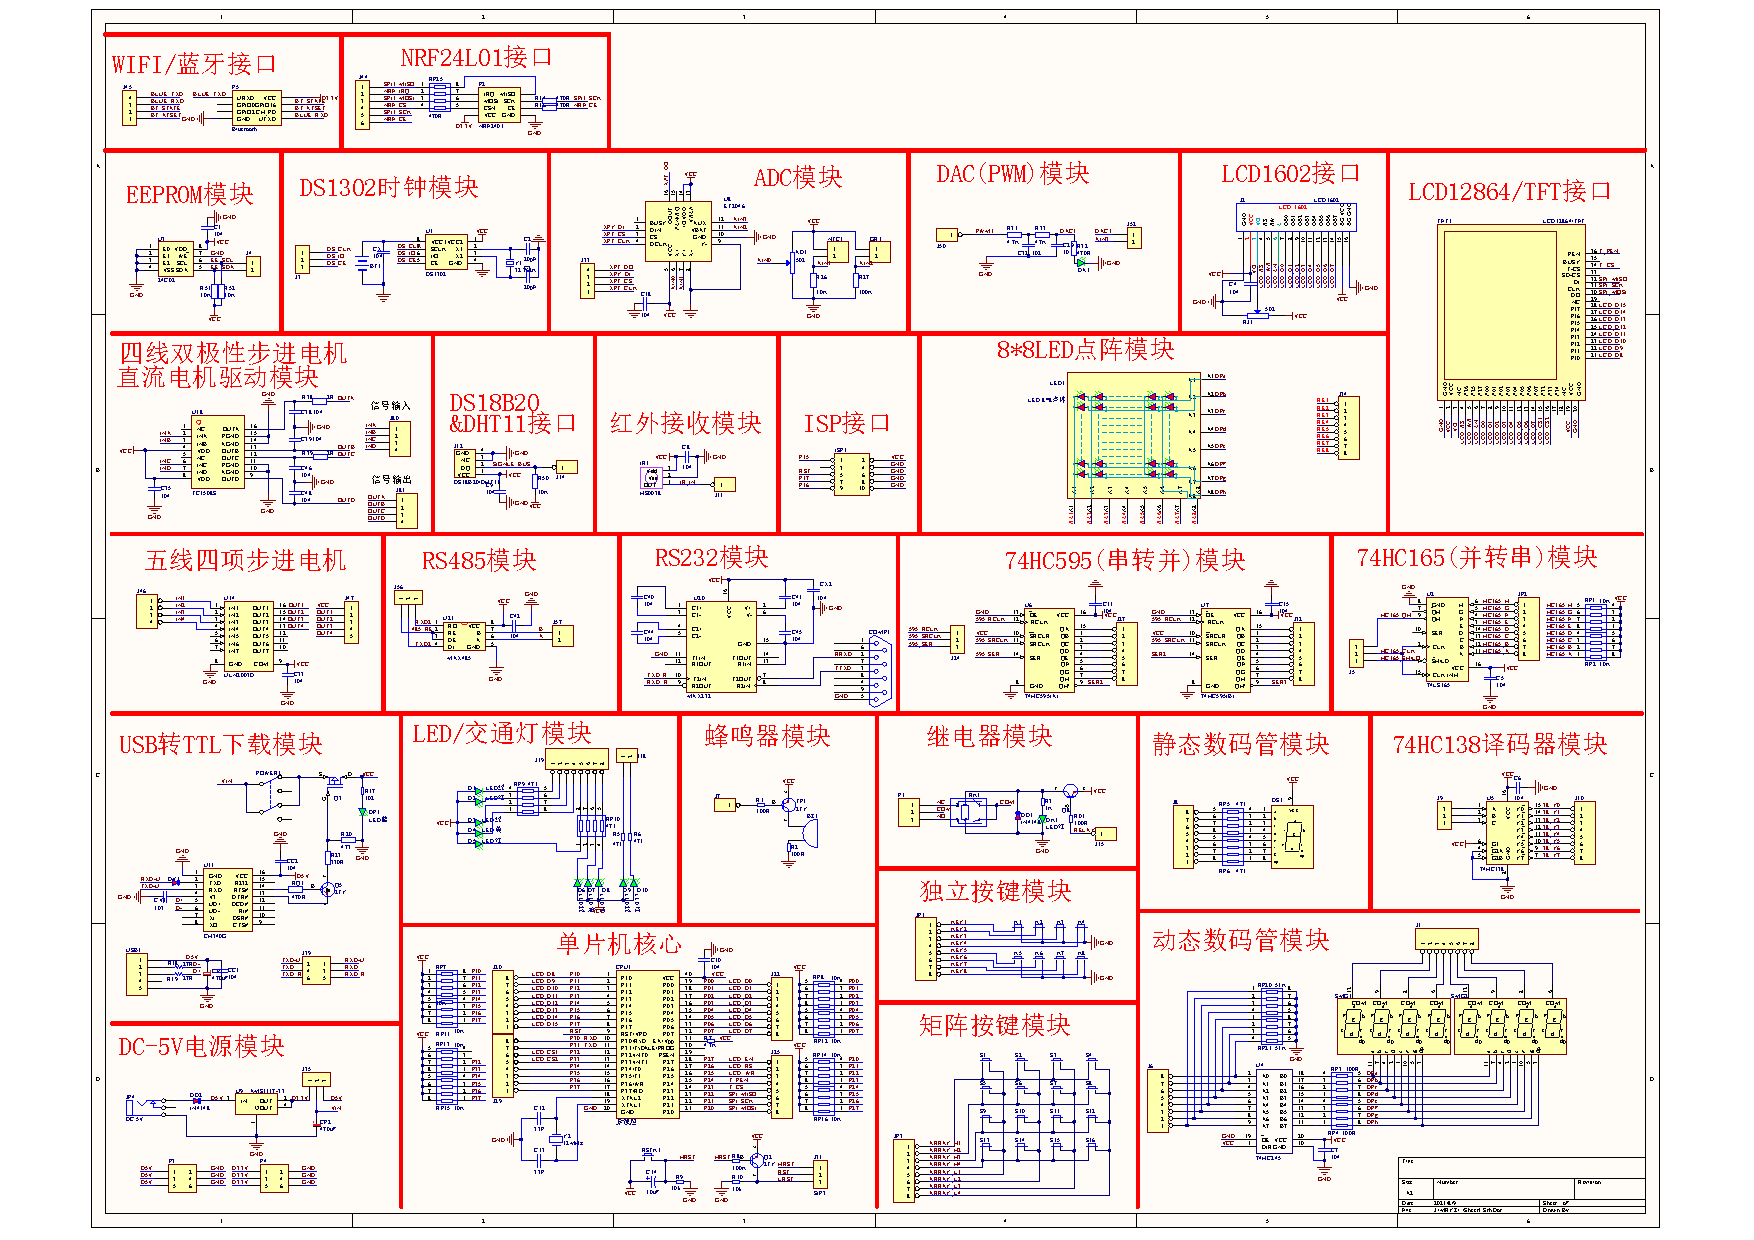
\includegraphics[scale=0.4]{Fig/开发板原理图.pdf}
		\caption{51单片机开发板原理图}\label{Fig.3}
	\end{figure}
	
	
	\subsection{51单片机开发板电路原理仿真图}	%3.2
	下面为根据51单片机开发板原理图所绘制的Poteus电路原理仿真图
	\begin{figure}[htbp]
		\centering
		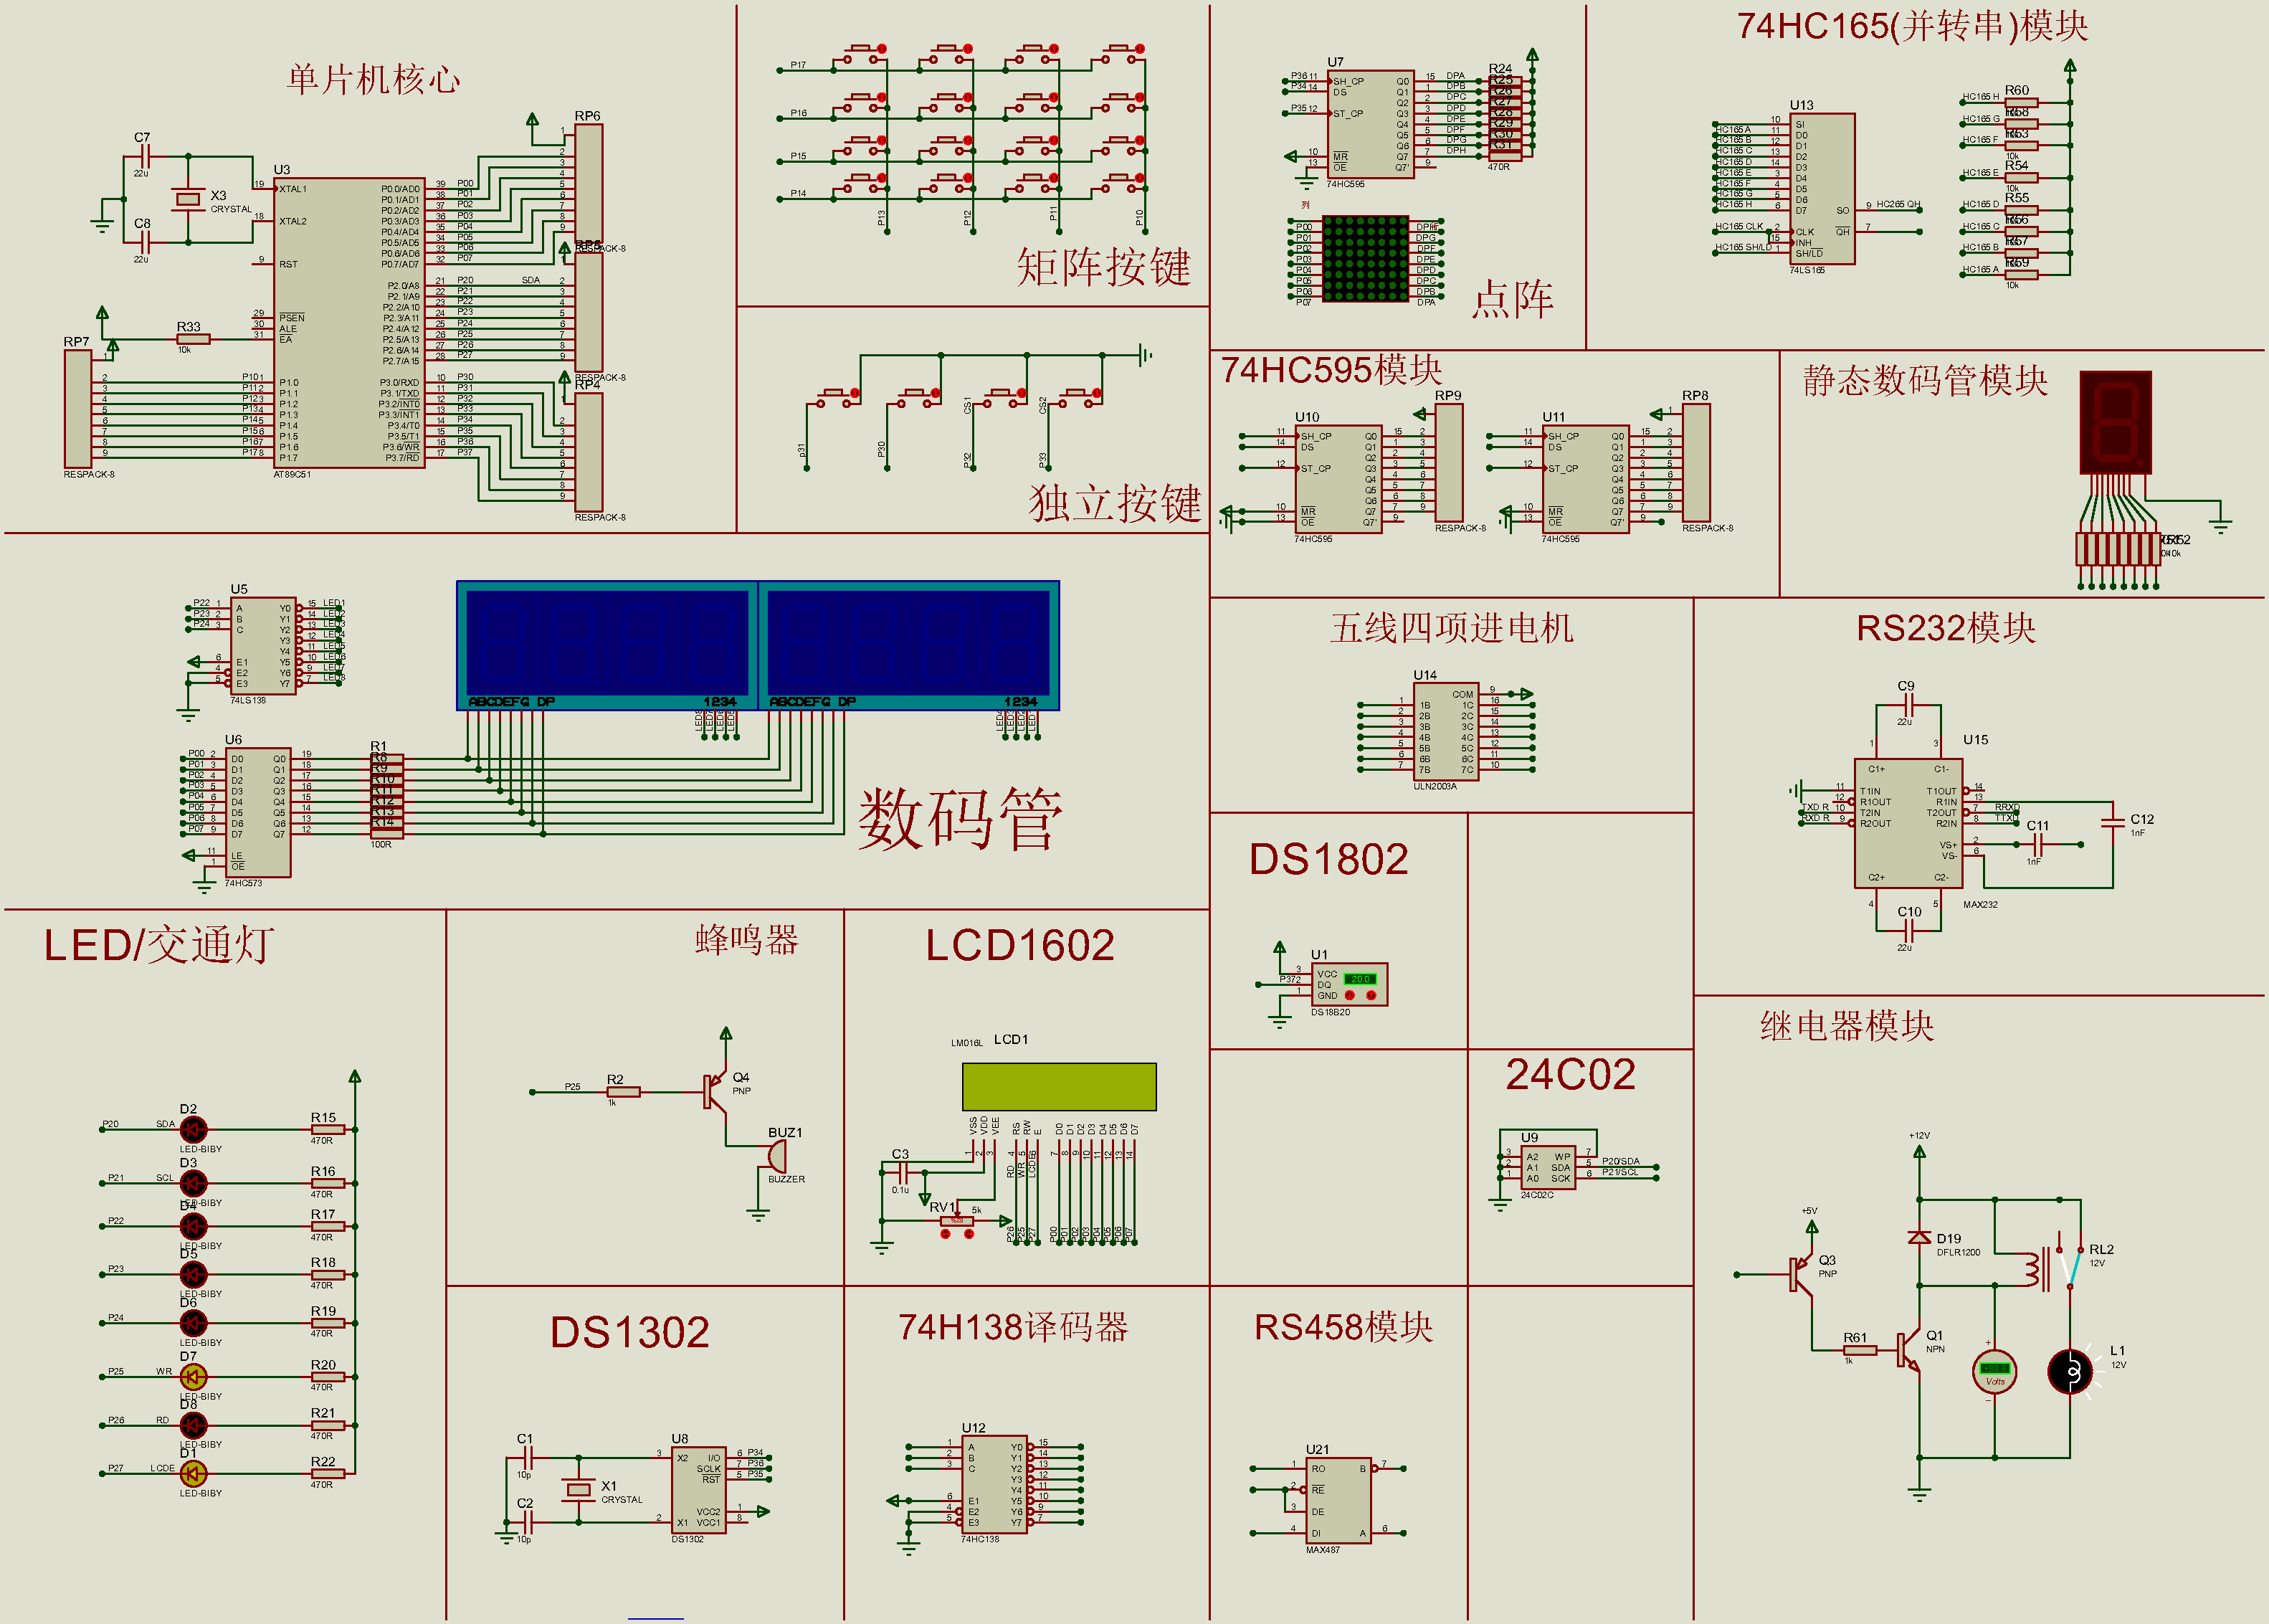
\includegraphics[scale=0.2]{Fig/学校51开发板仿真.PDF}
		\caption{51单片机开发板电路原理仿真图}\label{Fig.4}
	\end{figure}
	
	\subsection{主要电路原件原理及应用}		   %3.3
	
	
		\subsubsection{单片机核心}			      %3.3.1
		单片机,也称为微控制器(Microcontroller Unit, MCU),是一种集成电路芯片,它将微处理器(CPU)、存储器(包括程序存储器和数据存储器)、输入/输出(I/O)接口以及其他功能模块集成在一个芯片上。单片机的核心主要包括以下几个部分:
		
		中央处理单元(CPU):
		
		CPU是单片机的大脑,负责执行程序指令和处理数据。
		CPU通常包括算术逻辑单元(ALU)和控制单元(CU),用于执行算术和逻辑运算以及控制数据流。
		
		程序存储器:
		
		用于存储单片机执行的程序代码。
		可以是ROM(只读存储器)、PROM(可编程ROM)、EPROM(可擦写可编程ROM)或Flash存储器等类型。
		
		数据存储器:
		
		包括RAM(随机存取存储器)和特殊功能寄存器(SFR)。
		RAM用于临时存储数据和中间结果,而SFR用于存储控制和状态信息。
		输入/输出(I/O)接口:
		
		用于单片机与外部世界的通信,包括数字I/O和模拟I/O。
		数字I/O端口可以配置为输入或输出,用于控制或读取外部设备的状态。
		模拟I/O,如ADC(模拟/数字转换器)和DAC(数字/模拟转换器),用于处理模拟信号。
		
		定时器/计数器:
		
		用于测量时间间隔或计数事件的发生次数。
		可以用于产生精确的时间延迟、测量脉冲宽度或控制电机速度等。
		
		中断系统:
		
		允许单片机响应外部或内部事件,如按键按下、通信完成等。
		中断系统可以提高程序的响应速度和效率。
		
		串行通信接口:
		
		用于单片机与其他设备之间的串行数据传输。
		常见的串行通信协议包括SPI(串行外设接口)、I2C(交错式通信总线)和UART(通用异步接收/发送器)。
		
		时钟电路:
		
		为单片机提供时钟信号,是单片机运行的基础。
		可以是内部振荡器或外部时钟源。
		
		电源管理:
		
		包括低功耗模式,如睡眠模式或掉电模式,用于在不需要工作时减少能耗。
		
		其他功能模块:
		
		根据单片机的不同型号和应用需求,可能还包括其他功能模块,如PWM(脉冲宽度调制)控制器、RTC(实时时钟)等。
		\begin{figure}[htbp]
		\centering
		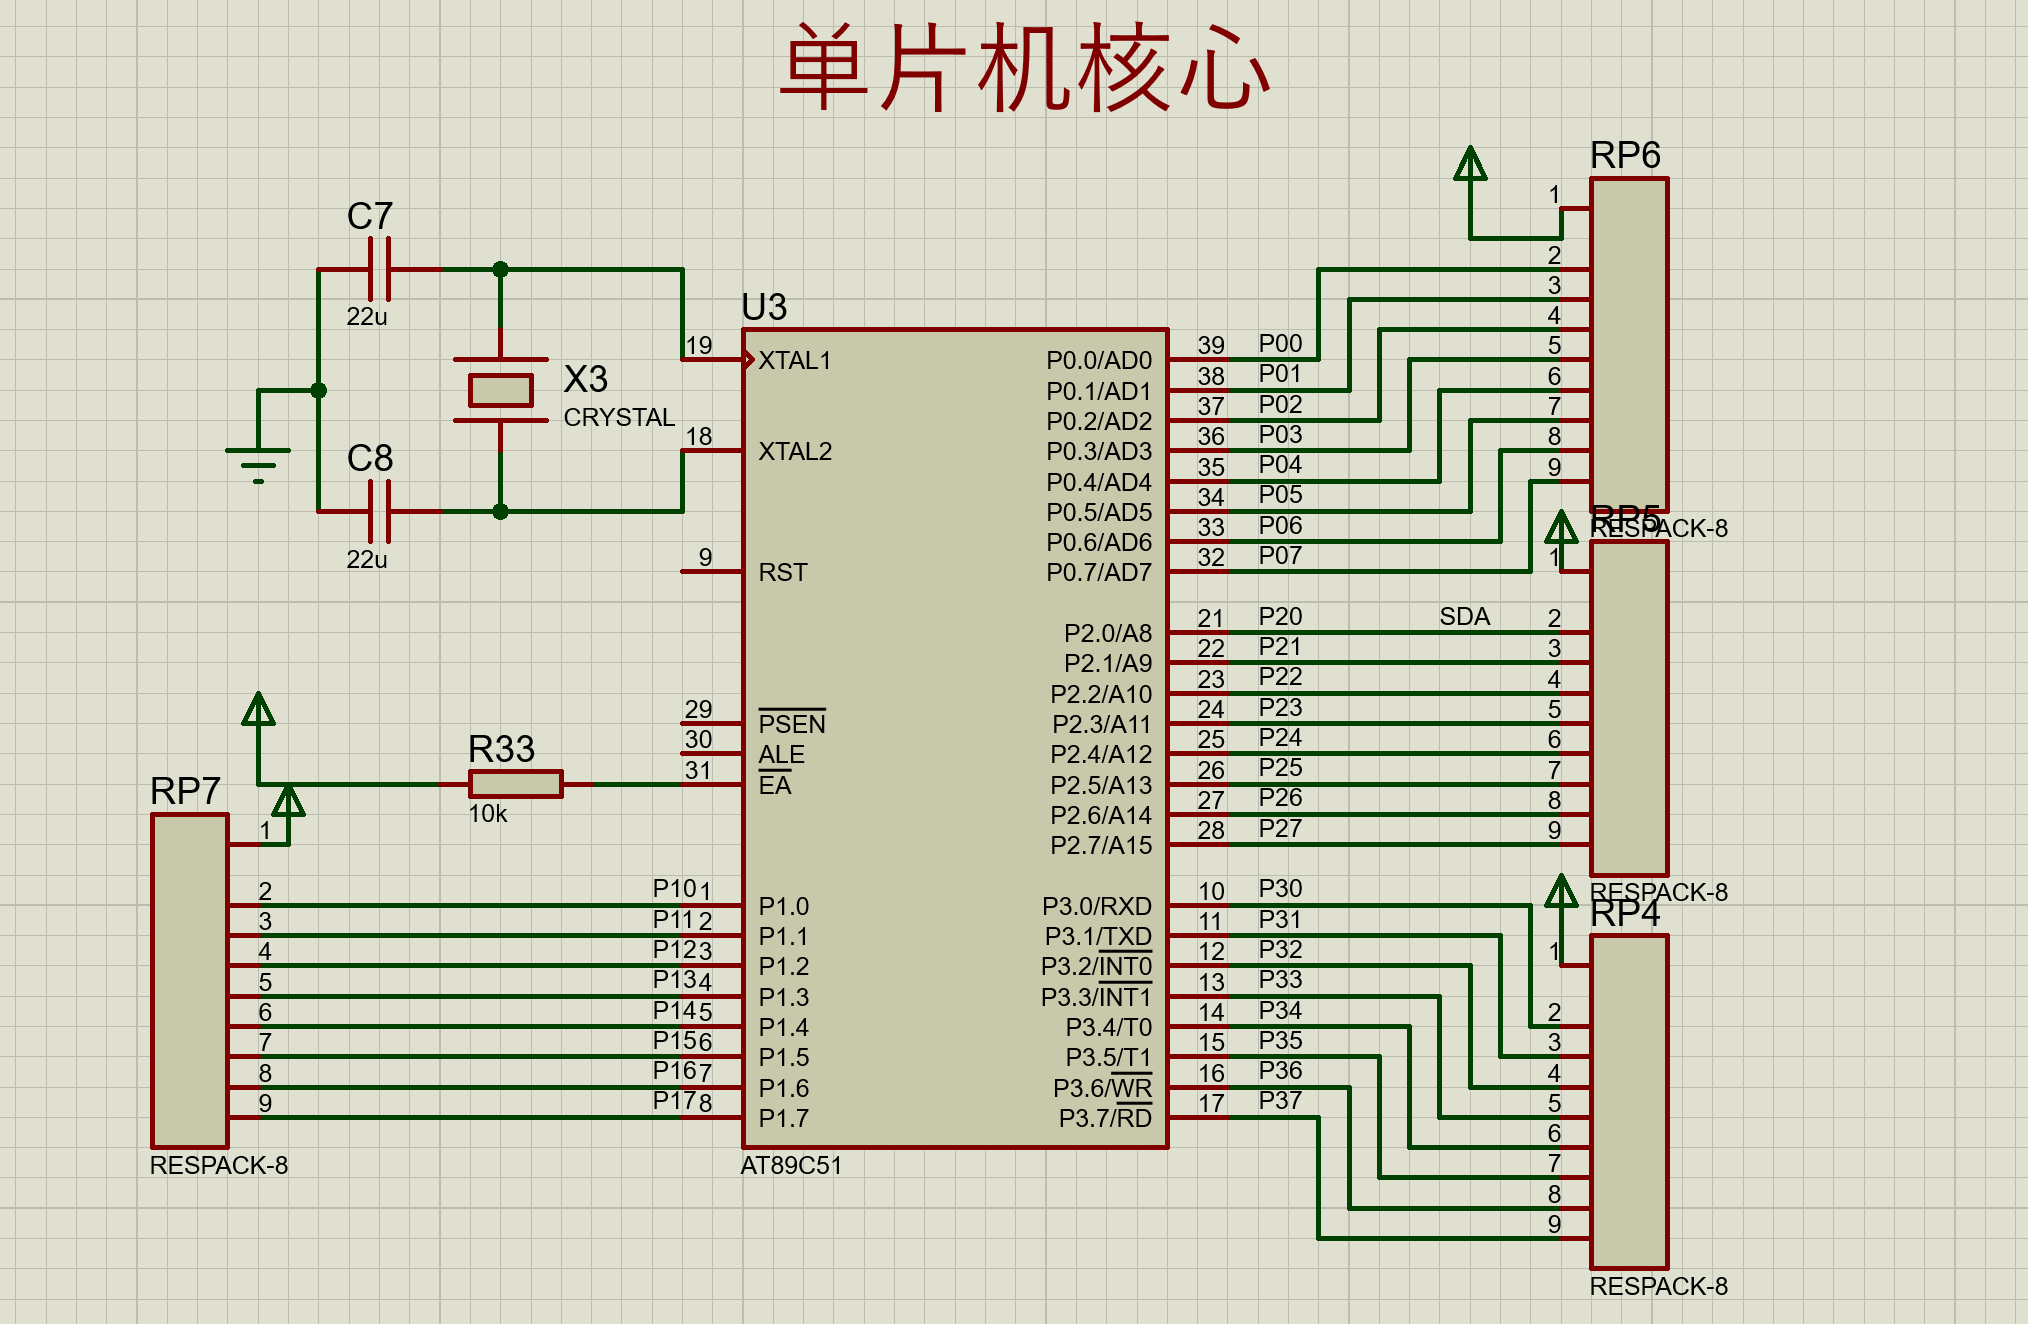
\includegraphics[scale=0.4]{Fig/单片机核心.png}
		\caption{单片机核心图}\label{Fig.6}
		\end{figure}


		\subsubsection{74HC595模块}				%3.3.2
		74HC595是一款由德州仪器(Texas Instruments)生产的8位串行输入、并行输出的移位寄存器。它广泛应用于各种数字电子项目中,如LED显示、数据存储和传输等。以下是74HC595的一些主要特性和功能:
		
		1. 串行数据输入:74HC595允许通过单个串行数据线输入数据,然后通过移位操作将数据分发到8个并行输出端。
		
		2. 存储寄存器:74HC595包含一个8位的存储寄存器,数据在移位操作后可以被存储在该寄存器中。
		
		3. 输出锁存器:数据可以被锁存到8位的输出锁存器中,从而驱动外部设备,如LED或继电器。
		
		4. 数据清零功能:74HC595具有数据清零功能,可以将移位寄存器和存储寄存器的数据清零。
		
		5. 输出使能控制:通过使能控制端,可以控制输出锁存器的输出状态,实现高阻态输出。
		
		6. 级联功能:74HC595设计有级联输出,允许多个74HC595芯片串联使用,扩展并行输出的位数。
		
		7. 应用场景:74HC595常用于LED点阵显示、数码管动态扫描、数据缓冲等场合。
		
		8. 引脚配置:
		- SER(Pin 14):串行数据输入端。
		- RCLK(Pin 12):存储寄存器时钟输入端,用于将移位寄存器的数据传输到存储寄存器。
		- SRCLK(Pin 11):移位寄存器时钟输入端,用于控制数据的移位。
		- OE(Pin 13):输出使能控制端,低电平有效。
		- MR(Pin 10):数据清零端,低电平有效。
		- QA-QH(Pin 1-8):8位并行输出端。
		- QH'(Pin 15):级联输出端,用于连接下一个74HC595的SER端。
		
		9. 工作原理:在移位模式下,数据通过SER端输入,每次SRCLK上升沿数据左移一位。当RCLK上升沿到来时,移位寄存器中的数据会被传输到存储寄存器,并从QA-QH端输出。
		
		10. 使用注意事项:在使用74HC595时,需要注意时钟信号的同步,以及数据输入和输出的时序,以确保数据正确传输和显示。
		
		74HC595以其灵活性和易用性,成为电子爱好者和工程师在数字电路设计中常用的组件之一。

		
		\begin{figure}[htbp]
			\centering
			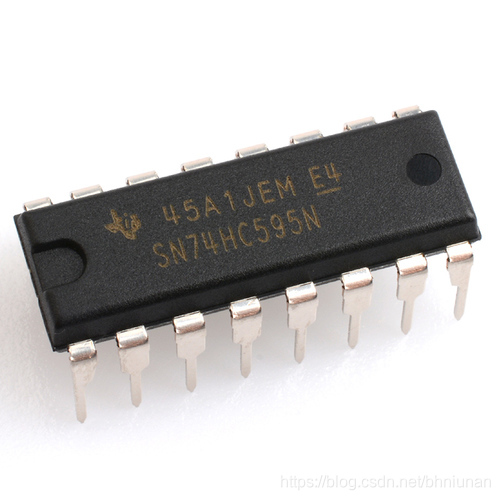
\includegraphics[scale=0.2]{Fig/74HC595(2).jpg}
			\caption{74HC595实物图}\label{Fig.9}
		\end{figure}
		
		
		\begin{figure}[htbp]
			\centering
			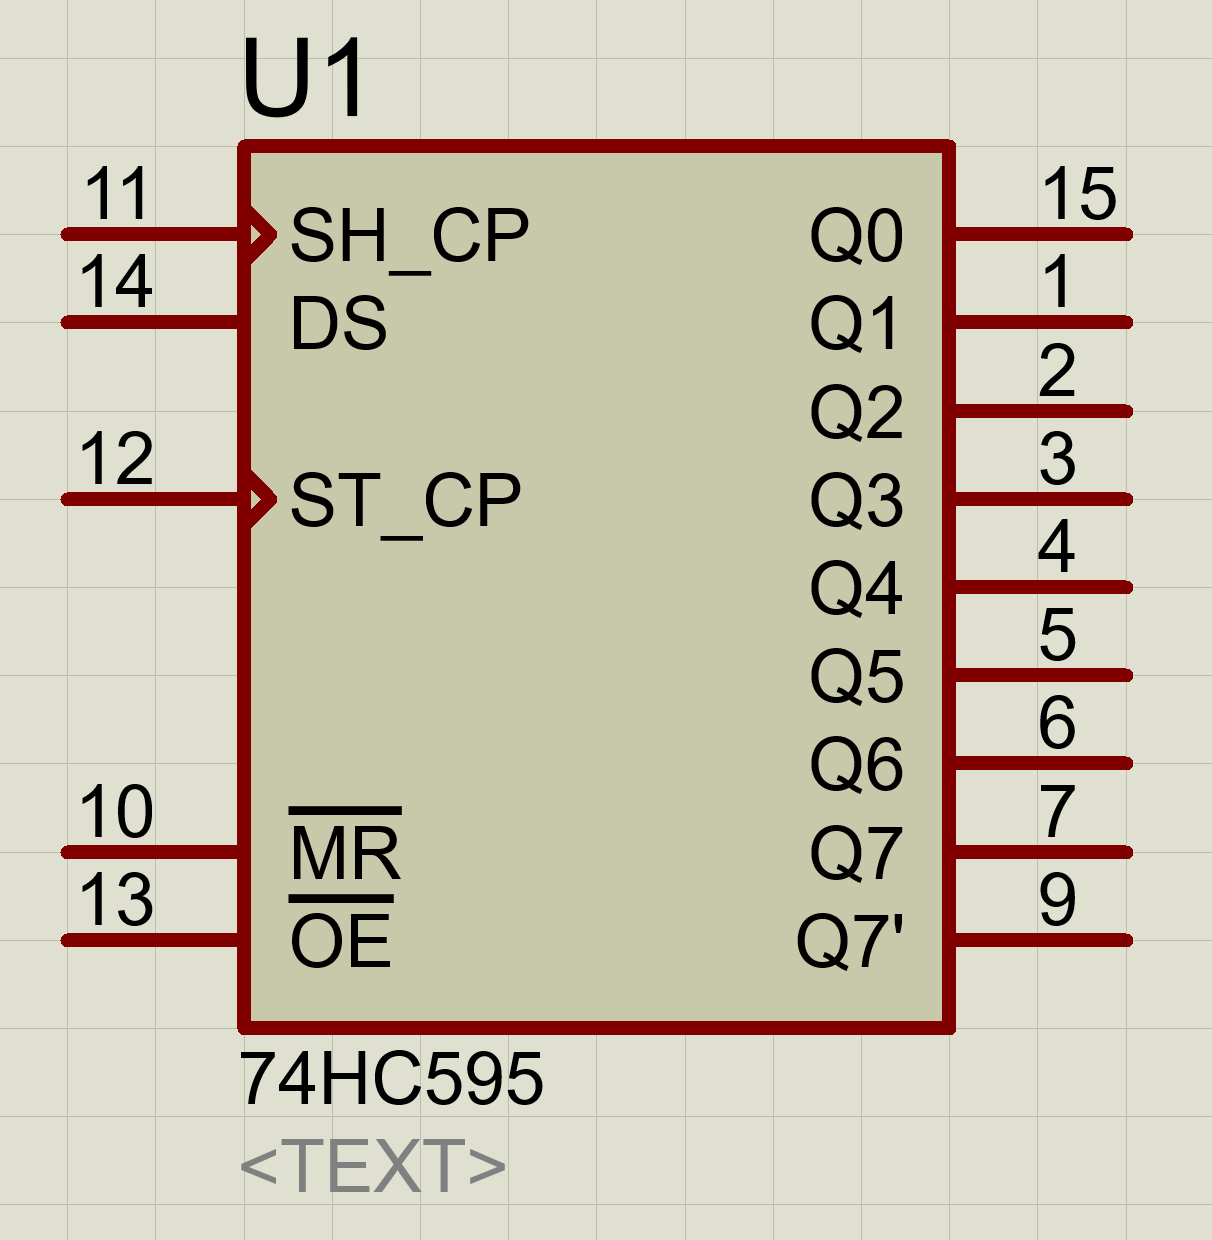
\includegraphics[scale=0.2]{Fig/74HC595.png}
			\caption{74HC595仿真图}\label{Fig.8}
		\end{figure}
		
		\begin{figure}[htbp]
			\centering
			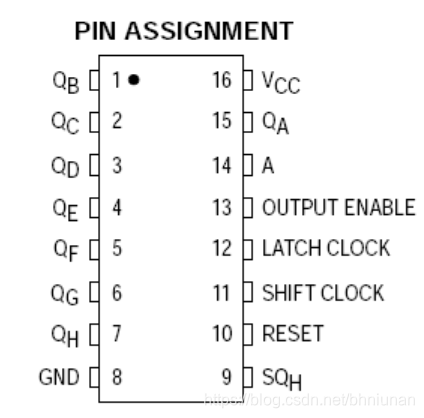
\includegraphics[scale=0.2]{Fig/74HC595(3).png}
			\caption{74HC595引脚图}\label{Fig.7}
		\end{figure}
		
		
		在一些电路中,我们需要对很多器件进行控制,但是我们的控制单元(比如单片机)的引脚数量有限,没有足够的引脚对器件进行控制。在这种情况下,采用串行转并行芯片是一个很好的选择,通过串行的数据输入实现对并行器件的控制。 74HC595通常是用来解决单片机I/O口不够用的情况。
		
		\begin{figure}[htbp]
			\centering
			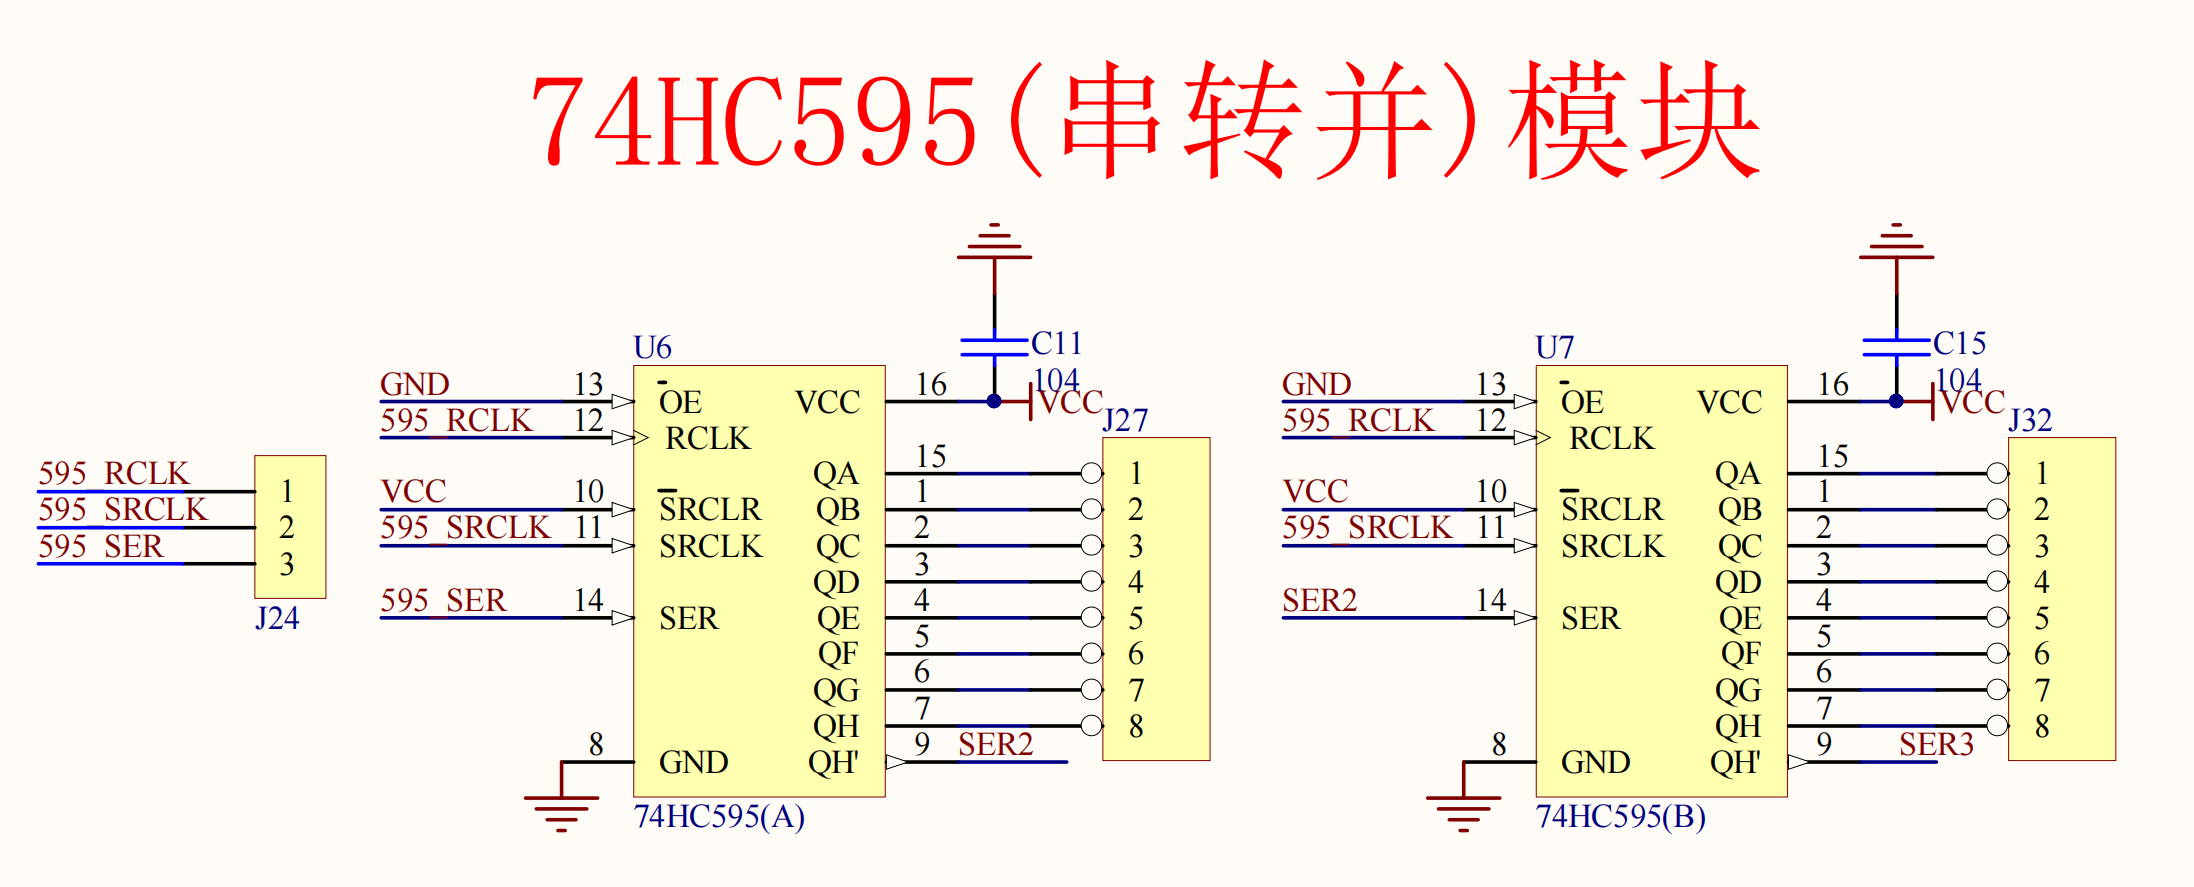
\includegraphics[scale=0.4]{Fig/74HC595串转并模块.png}
			\caption{74HC595串转并模块}\label{Fig.10}
		\end{figure}
		

	\subsubsection{74HC138模块}					%3.3.3
	一、74HC138简介
	74HC138是一款高速CMOS器件,74HC138引脚兼容低功耗肖特基TTL(LSTTL)系列。74HC138译码器可接受3位二进制加权地址输入(A0, A1和A2),并当使能时,提供8个互斥的低有效输出(Y0至Y7)。
	74HC138是一种译码器,译码是编码的逆过程,在编码时,每一种二进制代码,都赋予了特定的含义,即都表示了一个确定的信号或者对象。把代码状态的特定含义“翻译”出来的过程叫做译码,实现译码操作的电路称为译码器。
	74HC138的编码是000-111(八种),它们分别代表一种信号,要实现这些编码,只需要3根输入信号线;而74HC138这些编码所代表的含义,就是在8个输出中引脚中选出一个特殊的引脚,使其电平与其他7个不同,比如输出为01111111是输入为000的译码。所以,编码(被编的码)指的是有顺序规律,但没特殊含义的一种码;而译码(被译的码)指的是真正起作用的码。打个比方,ASCII码是一种编码,它的范围是0-127,光看这些码,我们无法得到任何有用的信息,但是,对他们进行译码后所得到的数据,我们就能轻易认出,比如ASCII编码97对应字符a,’a’就是译码。
	译码的例子还有很多,比如学号的译码就是学生身份信息,身份证的译码就是个人的信息等等。
	二、74HC138功能
	74HC138的功能在上一节已经提到,即将3位二进制(A0,A1和A2),译码成8种输出状态,并且一共有8个输出I/O,这8位输出的特点是:互斥(同时只有一位有效)、低有效(低电平表示有效,表示选中)。简单来说,74HC138实现了用3根线选择8根线(8选1)的功能。
	
	74HC138是一种3线至8线译码器/多路解复用器(Decoder/Demultiplexer),它能够根据3位二进制输入信号选择激活8个输出中的一个。以下是74HC138的一些关键特性和应用:
	
	1. 高速CMOS器件:74HC138采用高速CMOS技术,提供快速的响应时间和低功耗操作。
	
	2. 3位输入:该芯片接受3位二进制加权地址输入(A0, A1和A2),用于选择8个输出中的一个。
	
	3. 8个输出:74HC138提供8个互斥的低有效输出(Y0至Y7),当一个输出被激活时,其他输出保持高电平。
	
	4. 使能输入:具有两个低电平有效的使能输入端(G2A和G2B)和一个高电平有效的使能输入端(G1),这些使能端可以简化级联或数据接收。
	
	5. 应用场景:74HC138广泛应用于LED显示、服务器、白色家电、电力基础设施、楼宇自动化和工厂自动化等领域。
	
	6. 封装类型:74HC138提供多种封装选项,如SOIC、SSOP、PDIP、LCCC等,以适应不同的应用需求。
	
	7. 电气特性*74HC138的电气特性包括低功耗、宽工作电压范围(2V至6V)、高输出驱动能力(可驱动多达10个LSTTL负载)以及快速的传播延迟(典型值为15纳秒)。
	
	8. 设计指南:在设计时,需要注意输入和输出的电压水平,以及避免总线争用,因为74HC138的输出驱动能力较强,可能会引起电流超出最大限制。
	
	9. 数据表和技术支持:74HC138的数据表提供了详细的电气特性、引脚配置、功能块图和应用信息,同时德州仪器(TI)和其他供应商提供技术支持。
	
	10. ESD保护:74HC138具备ESD保护功能,能够在静电放电条件下提供一定程度的保护。
	
	74HC138的这些特性使其成为实现高效存储器译码或要求传输延迟时间短的数据传输系统中的理想选择。
	
	\begin{figure}[htbp]
		\centering
		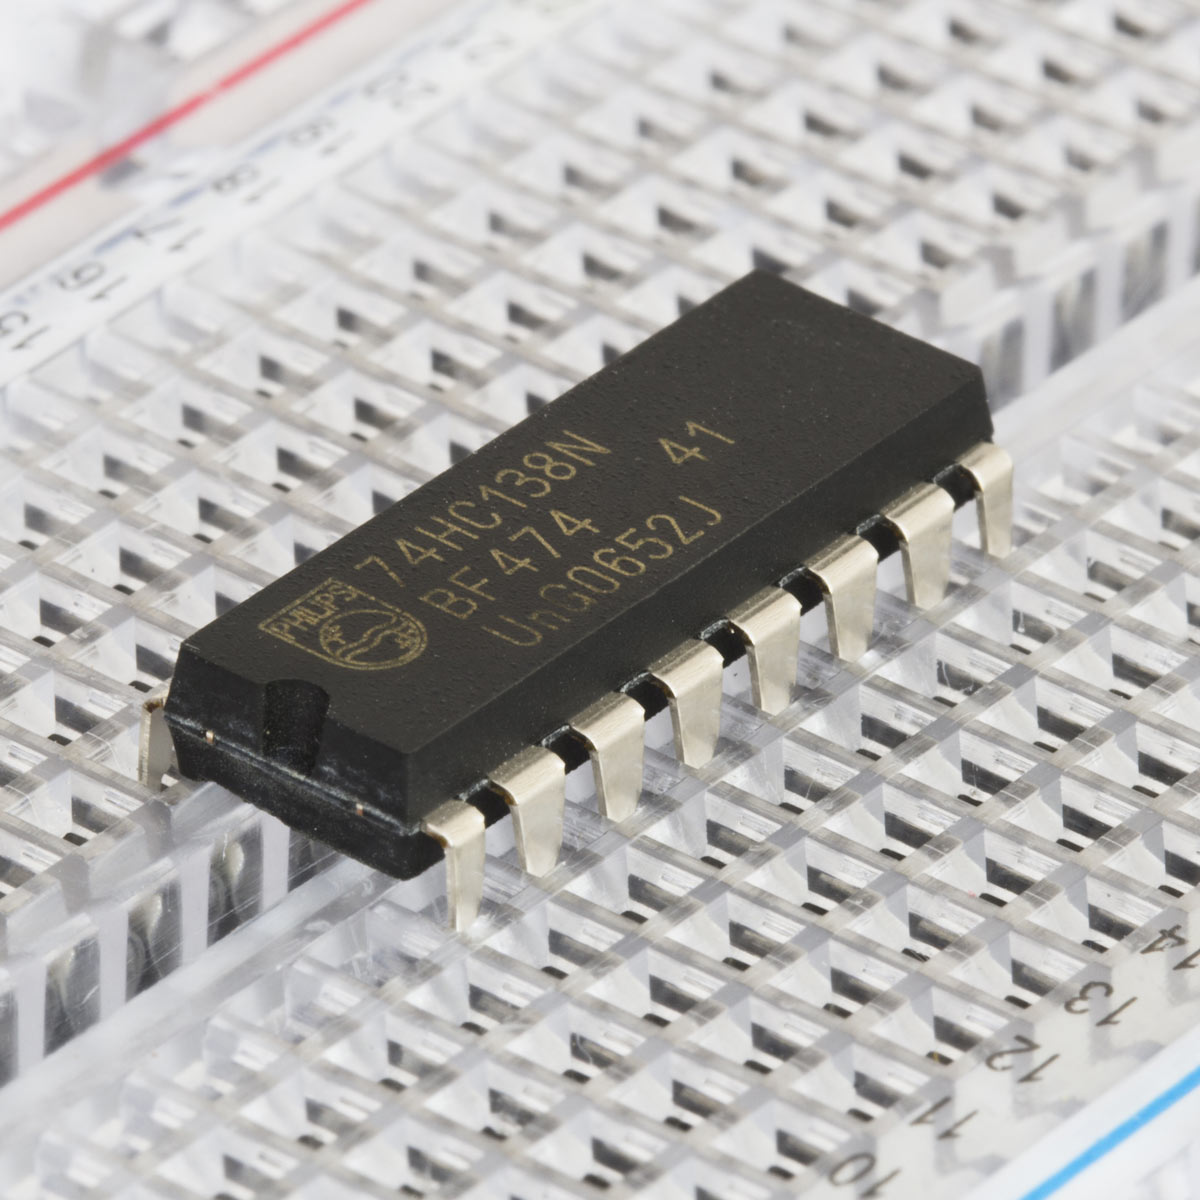
\includegraphics[scale=0.2]{Fig/74HC138(3).jpg}
		\caption{74HC138实物图}\label{Fig.15}
	\end{figure}
	
	\begin{figure}[htbp]
		\centering
		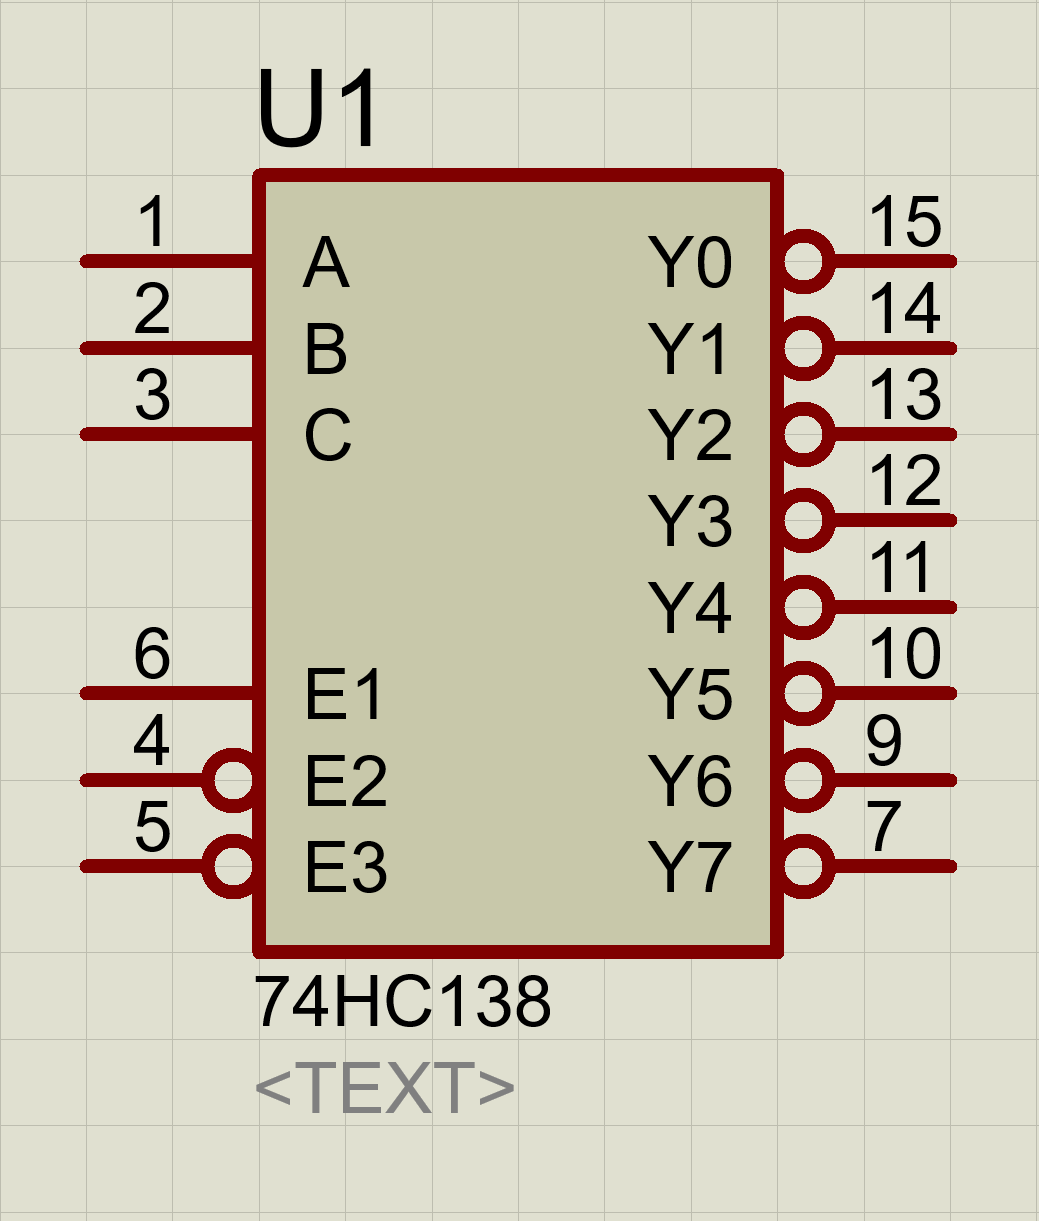
\includegraphics[scale=0.3]{Fig/74HC138.png}
		\caption{74HC138仿真图}\label{Fig.16}
	\end{figure}
	
	\begin{figure}[htbp]
		\centering
		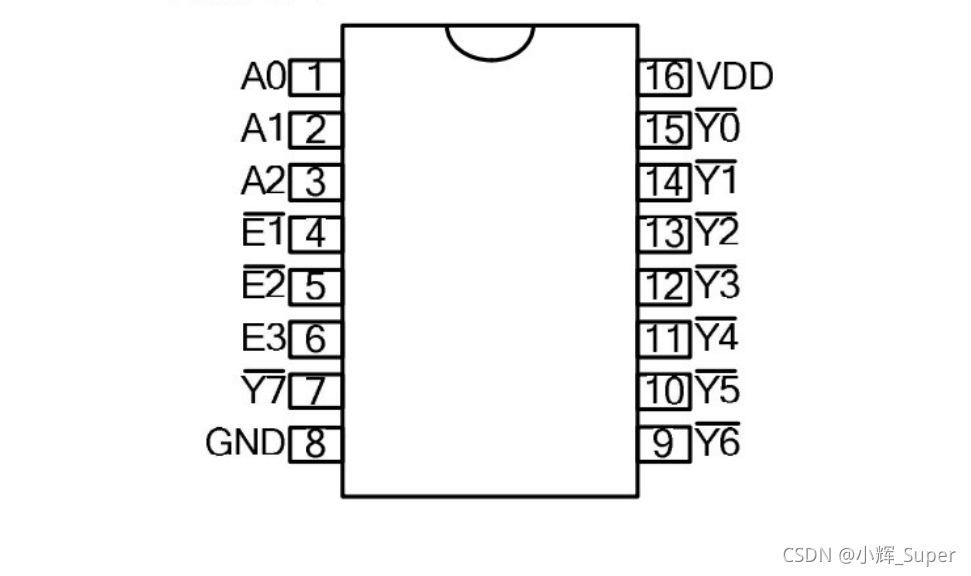
\includegraphics[scale=0.3]{Fig/74HC138(2).png}
		\caption{74HC138引脚图}\label{Fig.14}
	\end{figure}
	
	
	\begin{figure}[htbp]
		\centering
		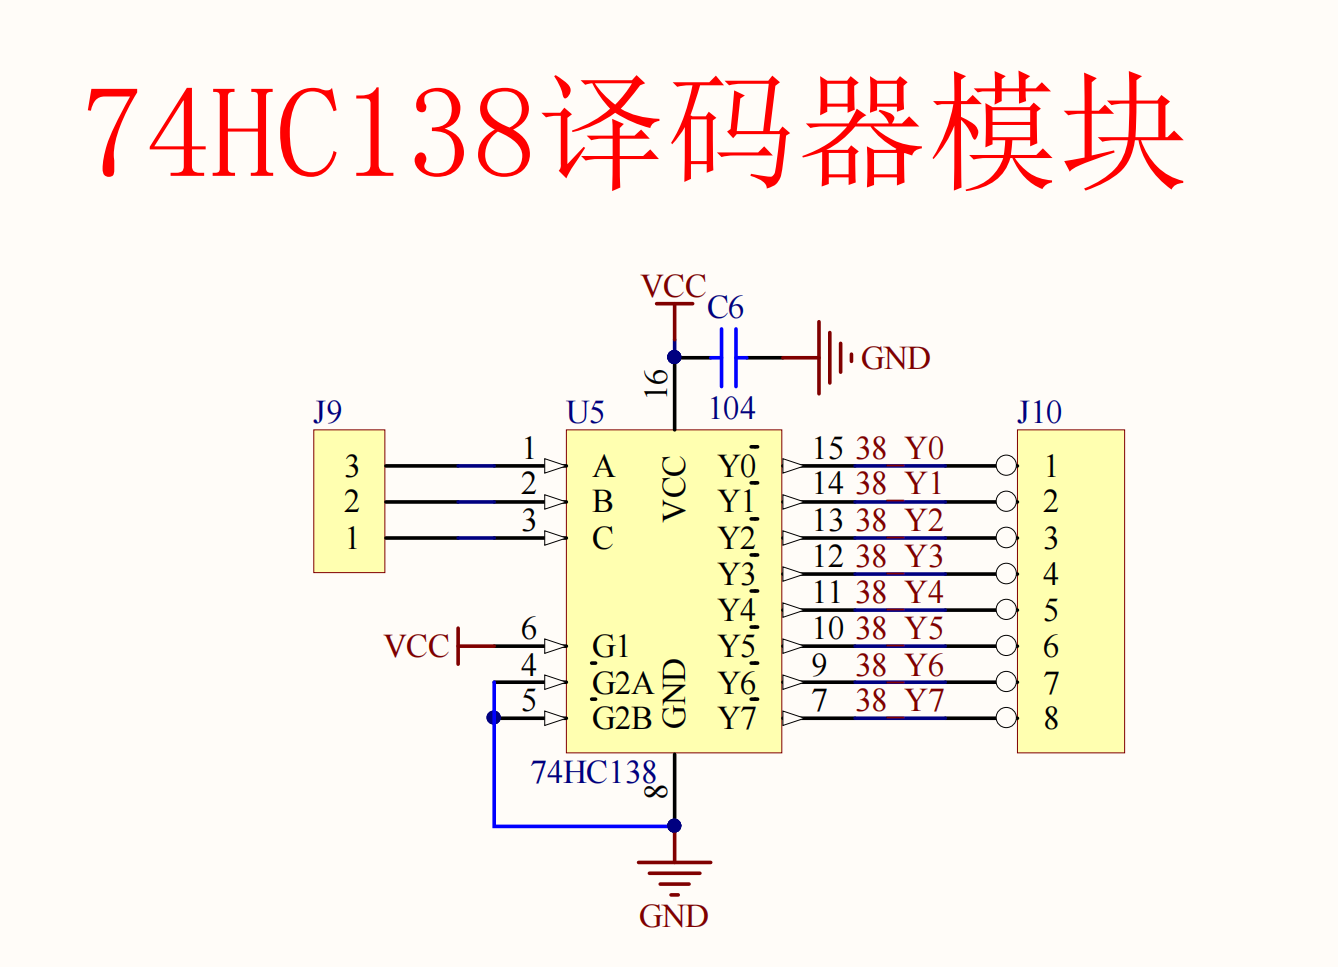
\includegraphics[scale=0.3]{Fig/38译码器模块.png}
		\caption{38译码器模块}\label{Fig.17}
	\end{figure}
	
	\subsubsection{动态数码管模块}					%3.3.4
	动态数码管通常指的是使用动态扫描技术的七段显示器(或数码管)系统。在数字电子和显示技术中,动态扫描是一种减少控制多位数显示所需的输入引脚数量的方法。下面是动态数码管的一些关键特点和应用:
	
	特点:
	
	1. 少引脚输出:通过时间复用技术,使用较少的输入引脚控制多个数码管或多位数字显示。
	
	2. 快速刷新:动态数码管通过快速切换显示的数字或段,利用人眼的视觉暂留效应,实现连续显示。
	
	3. 降低成本:由于减少了所需的引脚数量,可以降低控制系统的成本和复杂性。
	
	4. 驱动电路:通常需要晶体管或MOSFET等驱动元件来驱动每个段,尤其是当使用微控制器的I/O引脚直接驱动时。
	
	5. 控制方式:使用微控制器编程来控制不同段的显示,实现动态显示效果。
	
	应用:
	
数字时钟、计数器、仪器面板、家用电器、交通信号
	
	工作原理:
	
	动态数码管的工作原理基于以下步骤:
	
	1. 定义段:每个数码管由多个LED或LCD段组成,每个段可以独立控制。
	
	2. 定义位:在多位数码管中,每位数码管可以看作是一个独立的显示单元。
	
	3. 时间复用:通过快速轮流激活每一位数码管的各个段,实现动态显示。由于刷新速度快于人眼的感知能力,因此看起来所有数码管都是同时亮起的。
	
	4. 控制逻辑:使用微控制器编程来控制不同时间点上哪些段被激活,从而显示所需的数字或字符。
	
	设计考虑:
	
	刷新率:需要足够高的刷新率以避免显示闪烁。
	功耗管理:虽然单个LED或LCD段的功耗很低,但多位显示和高刷新率可能会增加总体功耗。
	显示稳定性:确保显示稳定,避免由于刷新不均匀导致的闪烁或重影。
	
	动态数码管是一种高效的显示解决方案,适用于需要显示多位数或字符的各种应用场景。通过精心设计和编程,可以实现清晰、稳定且具有吸引力的数字显示效果。
	
	\begin{figure}[htbp]
		\centering
		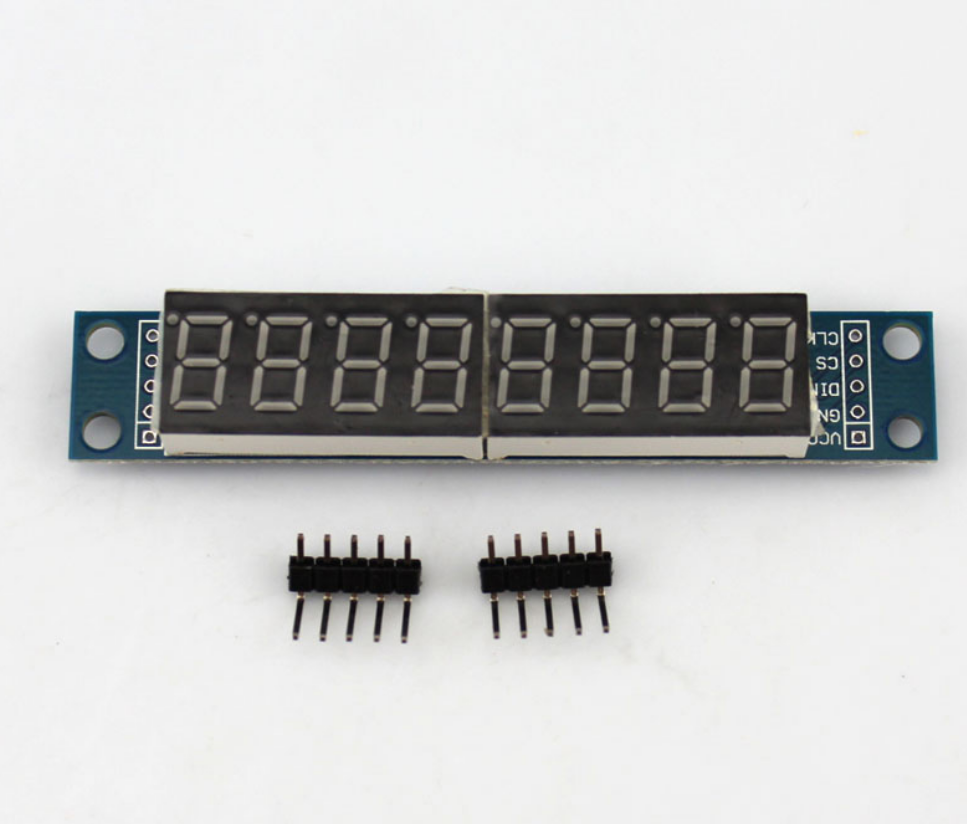
\includegraphics[scale=0.4]{Fig/动态数码管实物图.png}
		\caption{动态数码管实物图}\label{Fig.18}
	\end{figure}
	
	\begin{figure}[htbp]
		\centering
		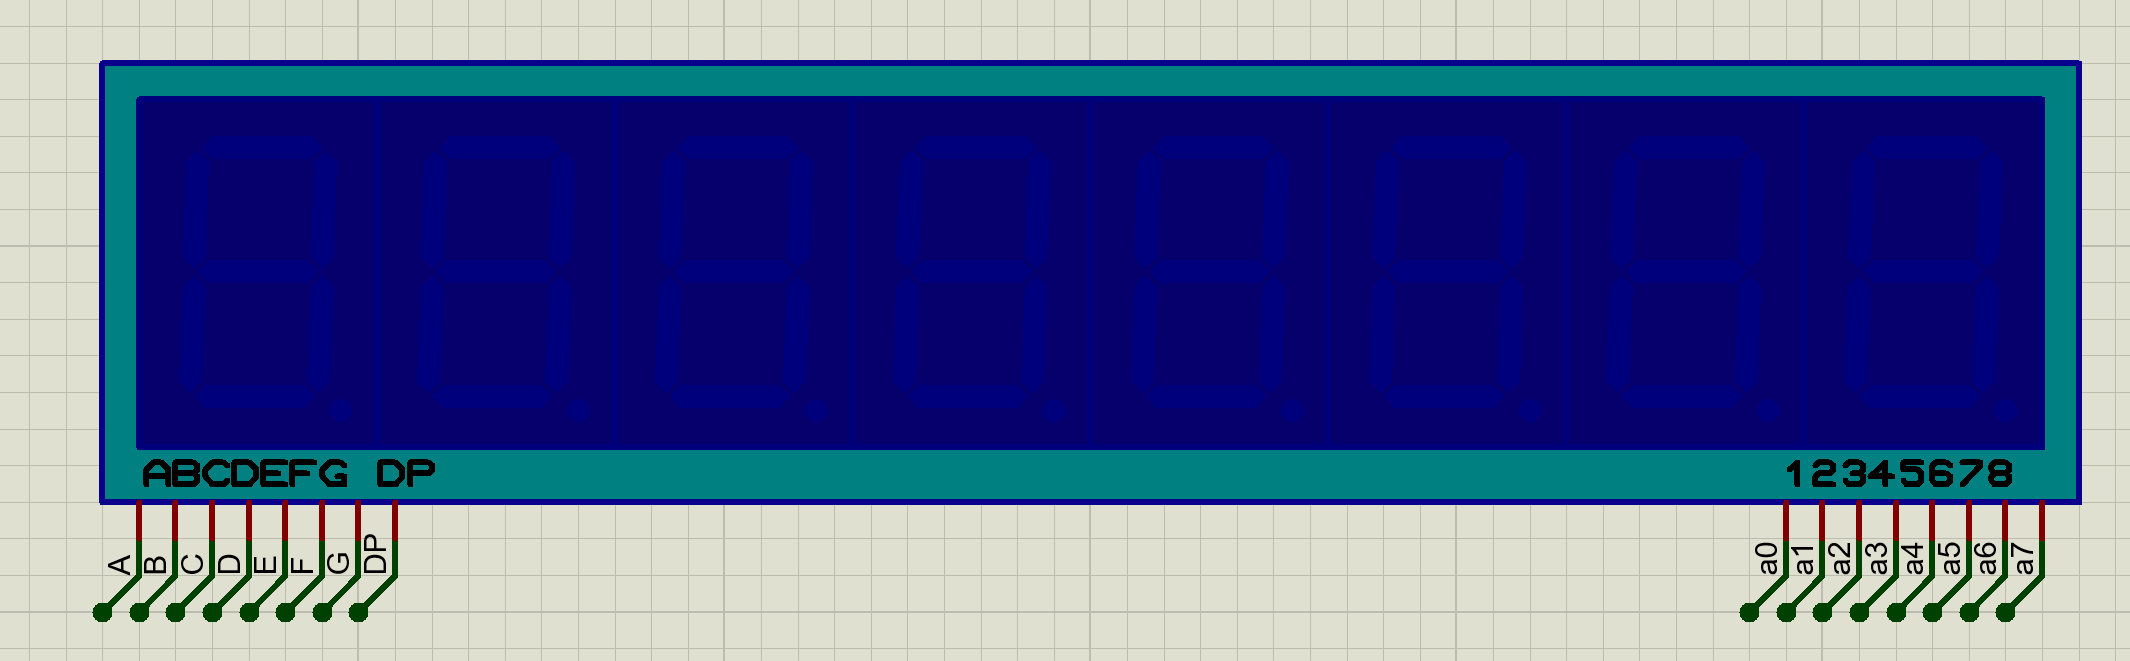
\includegraphics[scale=0.4]{Fig/7SEG-MPX.png}
		\caption{动态数码管仿真图}\label{Fig.19}
	\end{figure}
	
	
	\begin{figure}[htbp]
		\centering
		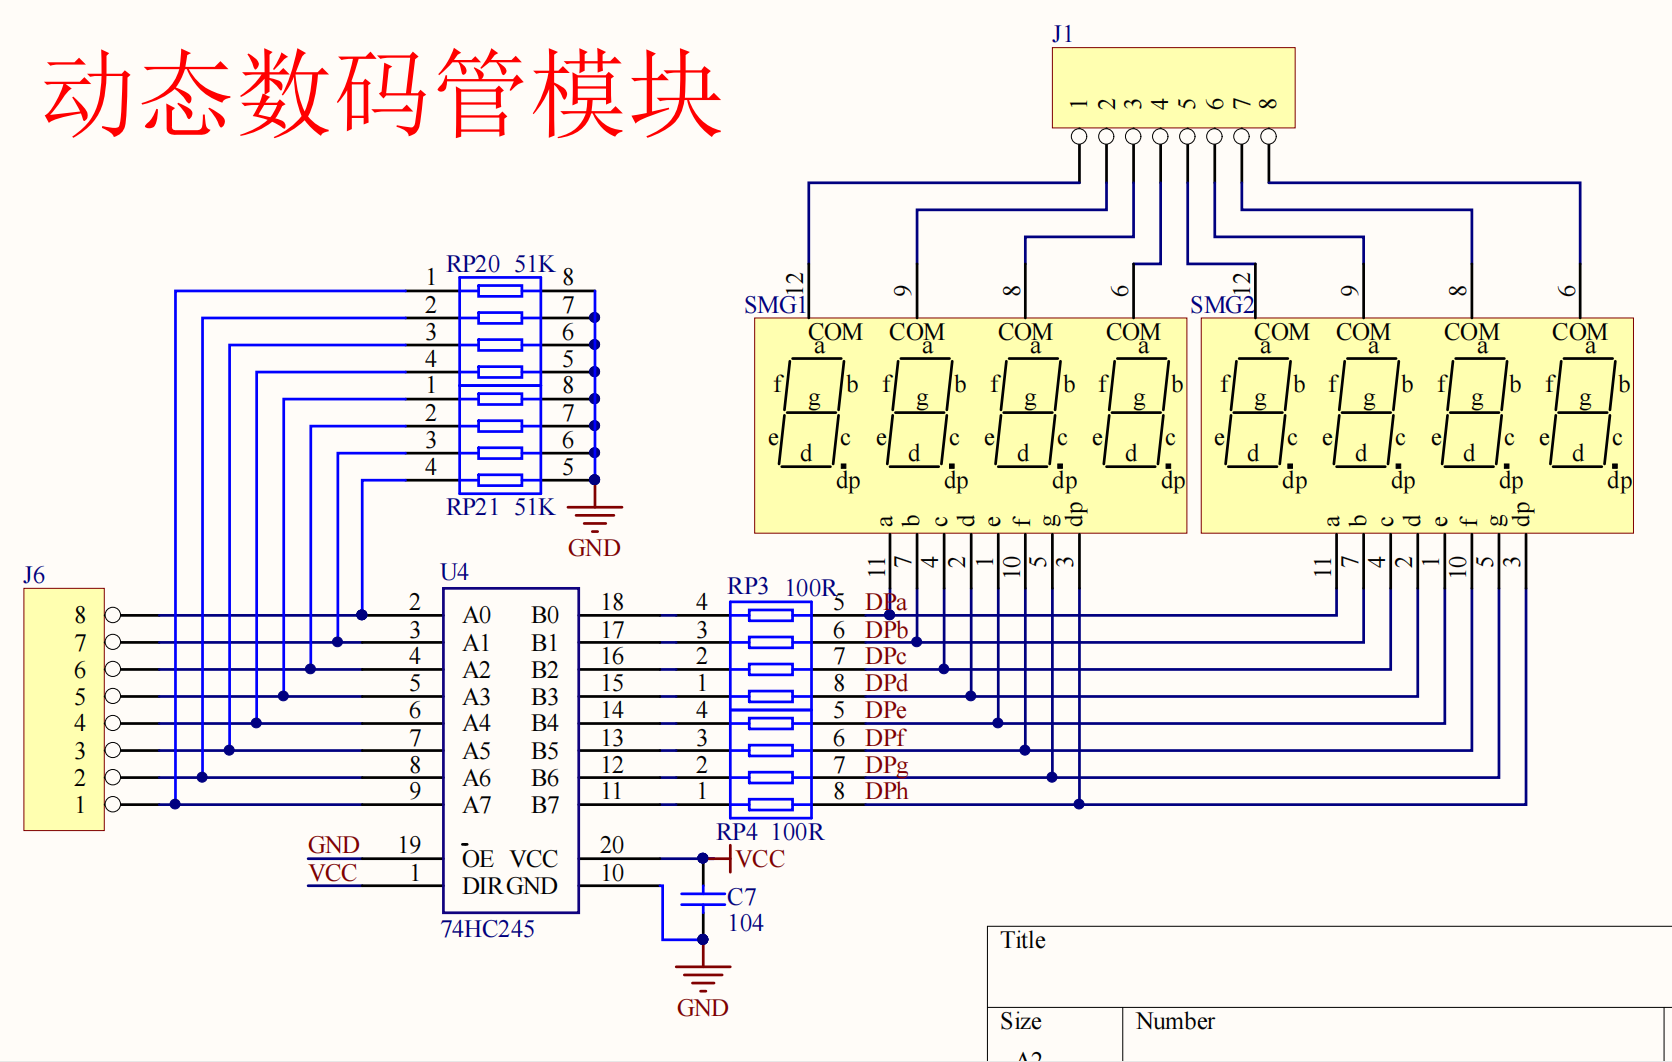
\includegraphics[scale=0.4]{Fig/动态数码管原理图.png}
		\caption{动态数码管原理图}\label{Fig.20}
	\end{figure}
	
\subsubsection{8x8点阵模块}						   %3.3.5
	8x8点阵(Dot Matrix)是一种显示技术,由64个LED(发光二极管)小灯或像素点组成,排列成8行8列的矩阵。这种点阵可以用来显示字母、数字、简单的图形和动画。以下是8x8点阵的一些关键特点和应用:
	
	特点:
	
	1. 模块化显示:由64个像素点组成,可以独立控制每个点的亮灭来形成不同的图案或文字。
	
	2. 灵活性高:可以编程显示各种字符、数字、图形和简单的动画。
	
	3. 低功耗:LED点阵的功耗相对较低,适合电池供电的应用。
	
	4. 易于控制:通常可以通过简单的接口如SPI或I2C与微控制器相连。
	
	5. 亮度调节:可以通过调节LED的电流或使用PWM(脉冲宽度调制)来控制亮度。
	
	6. 尺寸紧凑:8x8点阵模块通常体积较小,适合紧凑的空间。
	
	应用:
	
	1. 字符显示:显示数字、字母和一些特殊符号。
	
	2. 图形显示:显示简单的图形和图案。
	
	3. 信息板:用于显示状态信息、警告和通知。
	
	4. 游戏界面:在一些简单的电子游戏中作为游戏界面。
	
	5. 教育工具:用于教学演示,帮助理解数字和模拟信号的概念。
	
	6. 艺术装置:在艺术项目中创造动态视觉效果。
	
工作原理:
	
	1. 行驱动:8x8点阵的8行通常连接到微控制器的8个输出引脚,用于控制哪些行被激活。
	
	2. 列扫描:8列则通过另一个8个输出引脚进行控制,通过扫描列来点亮特定的LED。
	
	3. 动态刷新:通过快速刷新点阵(即快速切换LED的亮灭状态),利用人眼的视觉暂留效应,实现连续的显示效果。
	
	4. 编程控制:通过编程设置哪些行和列的LED被点亮,从而在点阵上形成所需的图案或文字。
	
	显示组件。通过创意编程,可以在点阵上实现丰富多彩的显示效果。
	
	\begin{figure}[htbp]
		\centering
		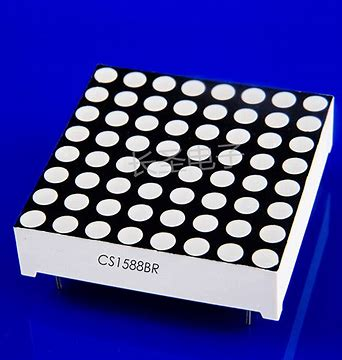
\includegraphics[scale=0.3]{Fig/点阵实物图.jpg}
		\caption{8x8点阵实物图}\label{Fig.21}
	\end{figure}
	
	\begin{figure}[htbp]
		\centering
		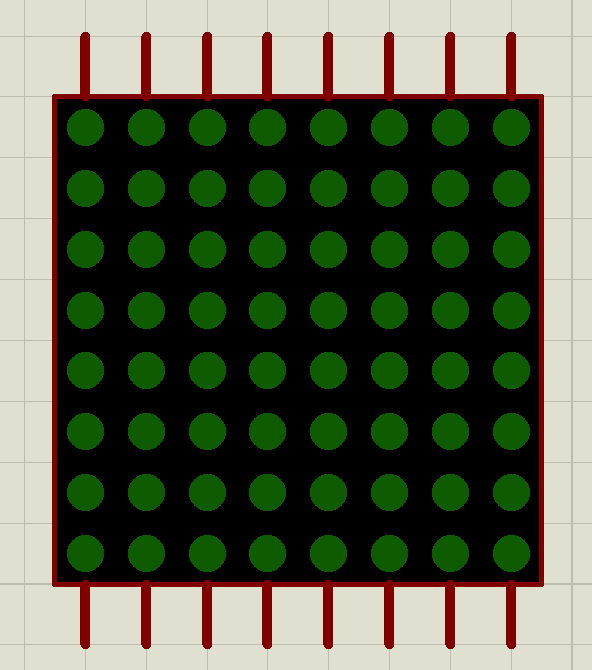
\includegraphics[scale=0.3]{Fig/点阵仿真图.png}
		\caption{8x8点阵仿真图}\label{Fig.22}
	\end{figure}
	
	
	\begin{figure}[htbp]
		\centering
		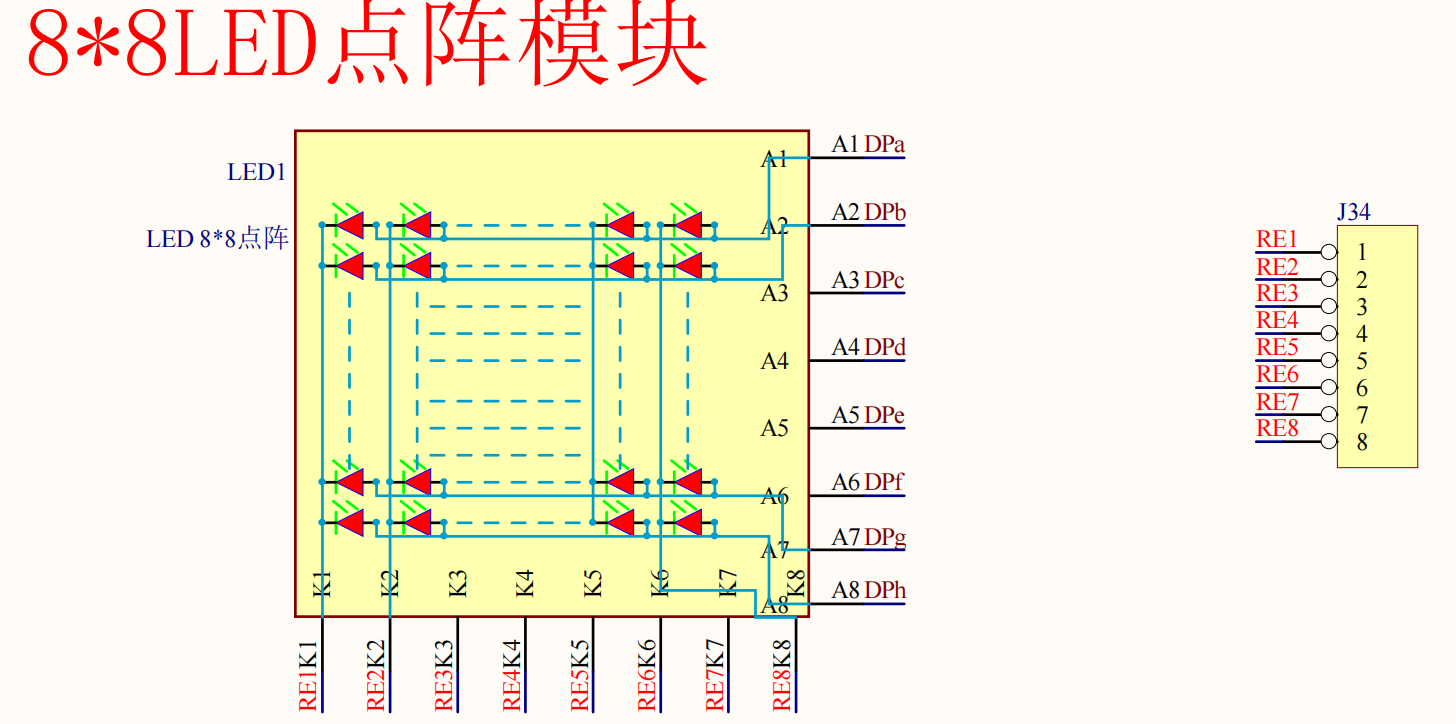
\includegraphics[scale=0.3]{Fig/点阵原理图.png}
		\caption{8x8点阵原理图}\label{Fig.23}
	\end{figure}
	
	\subsubsection{传感器DS18B20模块}			  %3.3.6
	DS18B20是一款由Maxim Integrated(前Dallas Semiconductor)生产的数字温度传感器,它具有以下特点:
	
	1. 高精度:DS18B20能够提供9到12位的可编程分辨率,最高可达±0.5°C的精度。
	
	2. 宽温度范围:测量温度范围从-55°C到+125°C。
	
	3. 数字输出:传感器使用1-Wire通信协议进行数据传输,这意味着它只需要一个数据线和地线即可工作,简化了布线。
	
	4. 多点能力:在同一个1-Wire总线上可以连接多个DS18B20传感器,实现多点温度监测。
	
	5. 非易失性存储:DS18B20具有内部存储空间,可以存储配置和温度警报触发值。
	
	6. 温度报警:可以设置温度报警阈值,当温度超过这些阈值时,传感器会触发一个报警信号。
	
	7. 小尺寸封装:DS18B20通常采用TO-92、SOIC或PDIP封装,适合紧凑的空间。
	
	8. 宽电压范围:传感器可以在多种电压下工作,包括3.0V至5.5V的电源电压。
	
	9. 易于编程:可以通过编程设置分辨率、温度报警阈值等参数。
	
	10. 应用广泛:适用于工业、科研、环境监测等多种场合的温度测量。
	
	DS18B20的工作原理基于温度变化导致传感器内部的半导体材料电阻值变化,通过内部电路将这种变化转换为数字信号输出。它使用1-Wire通信协议,这种协议允许多个设备共享同一通信线路,并通过唯一的ROM序列号进行识别。
	
	在实际应用中,DS18B20可以通过微控制器或其他具有1-Wire接口的设备进行控制和数据读取。用户可以通过编程发送指令来读取温度值、设置分辨率、配置报警阈值等。
	
	DS18B20的这些特性使其成为在需要精确温度测量和控制的应用中的理想选择。
	
	
	\begin{figure}[htbp]
		\centering
		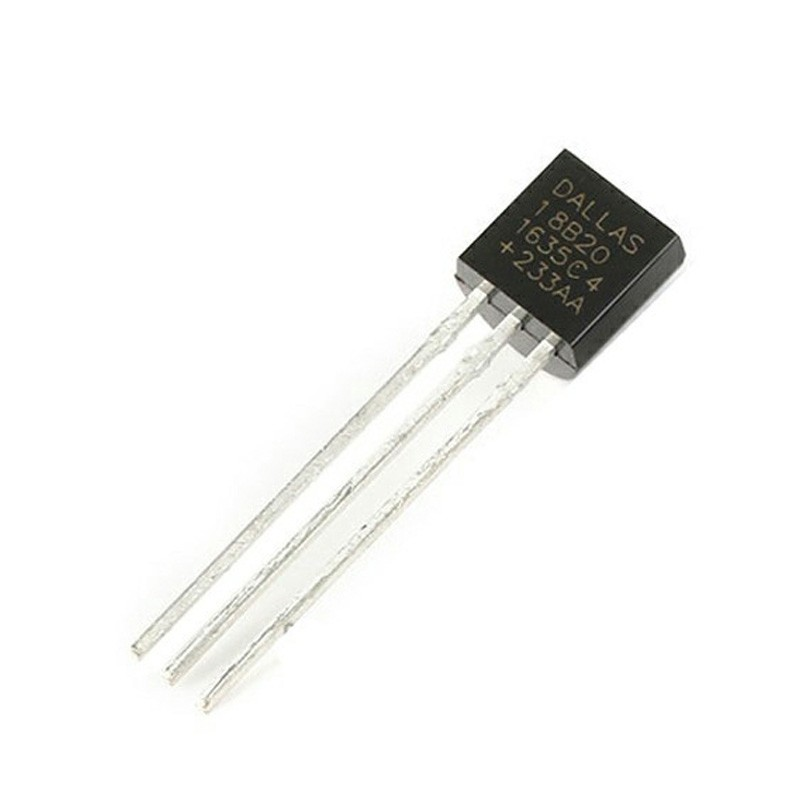
\includegraphics[scale=0.1]{Fig/DS18B.jpg}
		\caption{DS18B20实物图}\label{Fig.30}
	\end{figure}
	
	\begin{figure}[htbp]
		\centering
		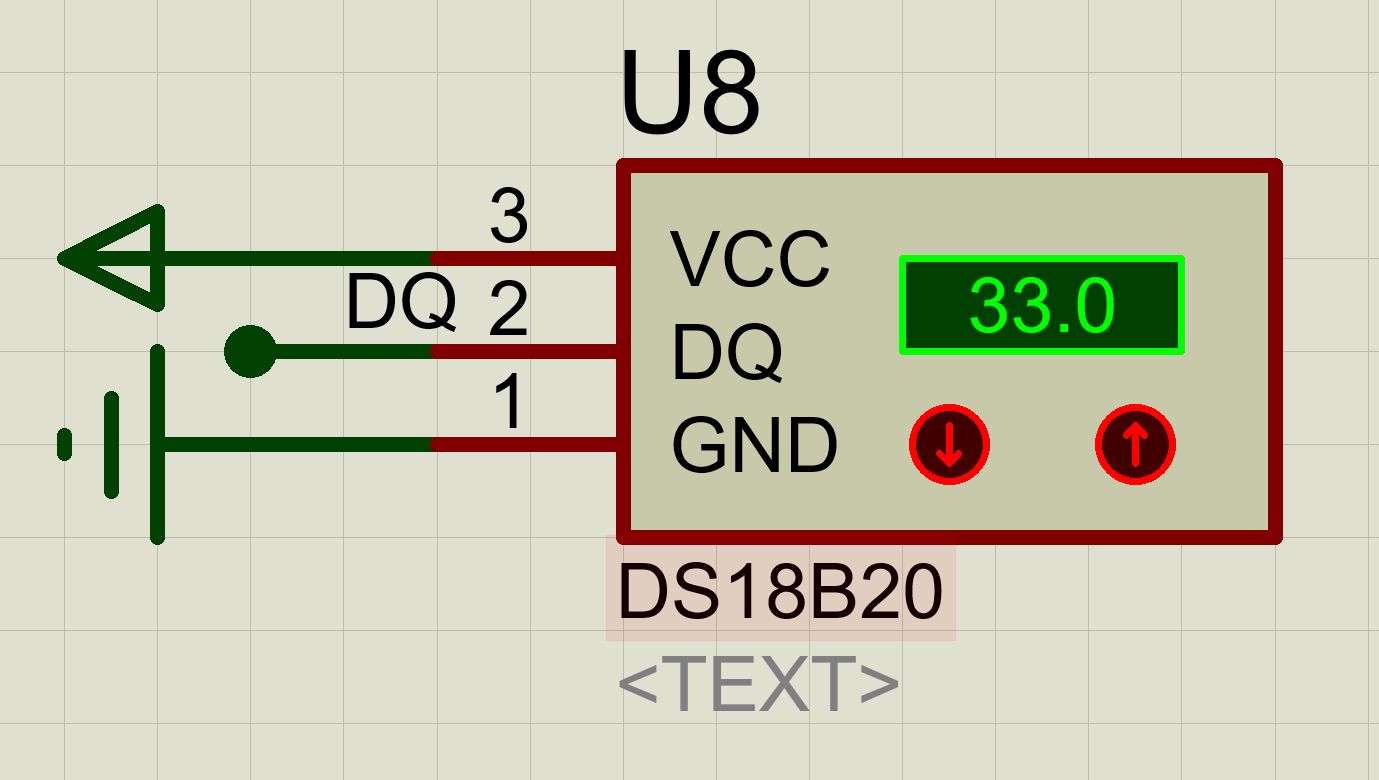
\includegraphics[scale=0.3]{Fig/DS18.png}
		\caption{DS18B20仿真图}\label{Fig.31}
	\end{figure}
	
	
	\begin{figure}[htbp]
		\centering
		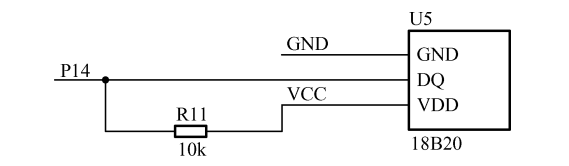
\includegraphics[scale=0.3]{Fig/DS18B2.png}
		\caption{DS18B20原理图}\label{Fig.32}
	\end{figure}
	
	
\section{项目实现}					 		%四
	
	
	\subsection{电路实现}                       %4.1
	由51单片机开发板原理图及各个原部件和模块原理可以绘制本项目的Proteus仿真图如下:
	
	\begin{figure}[htbp]
	\centering
	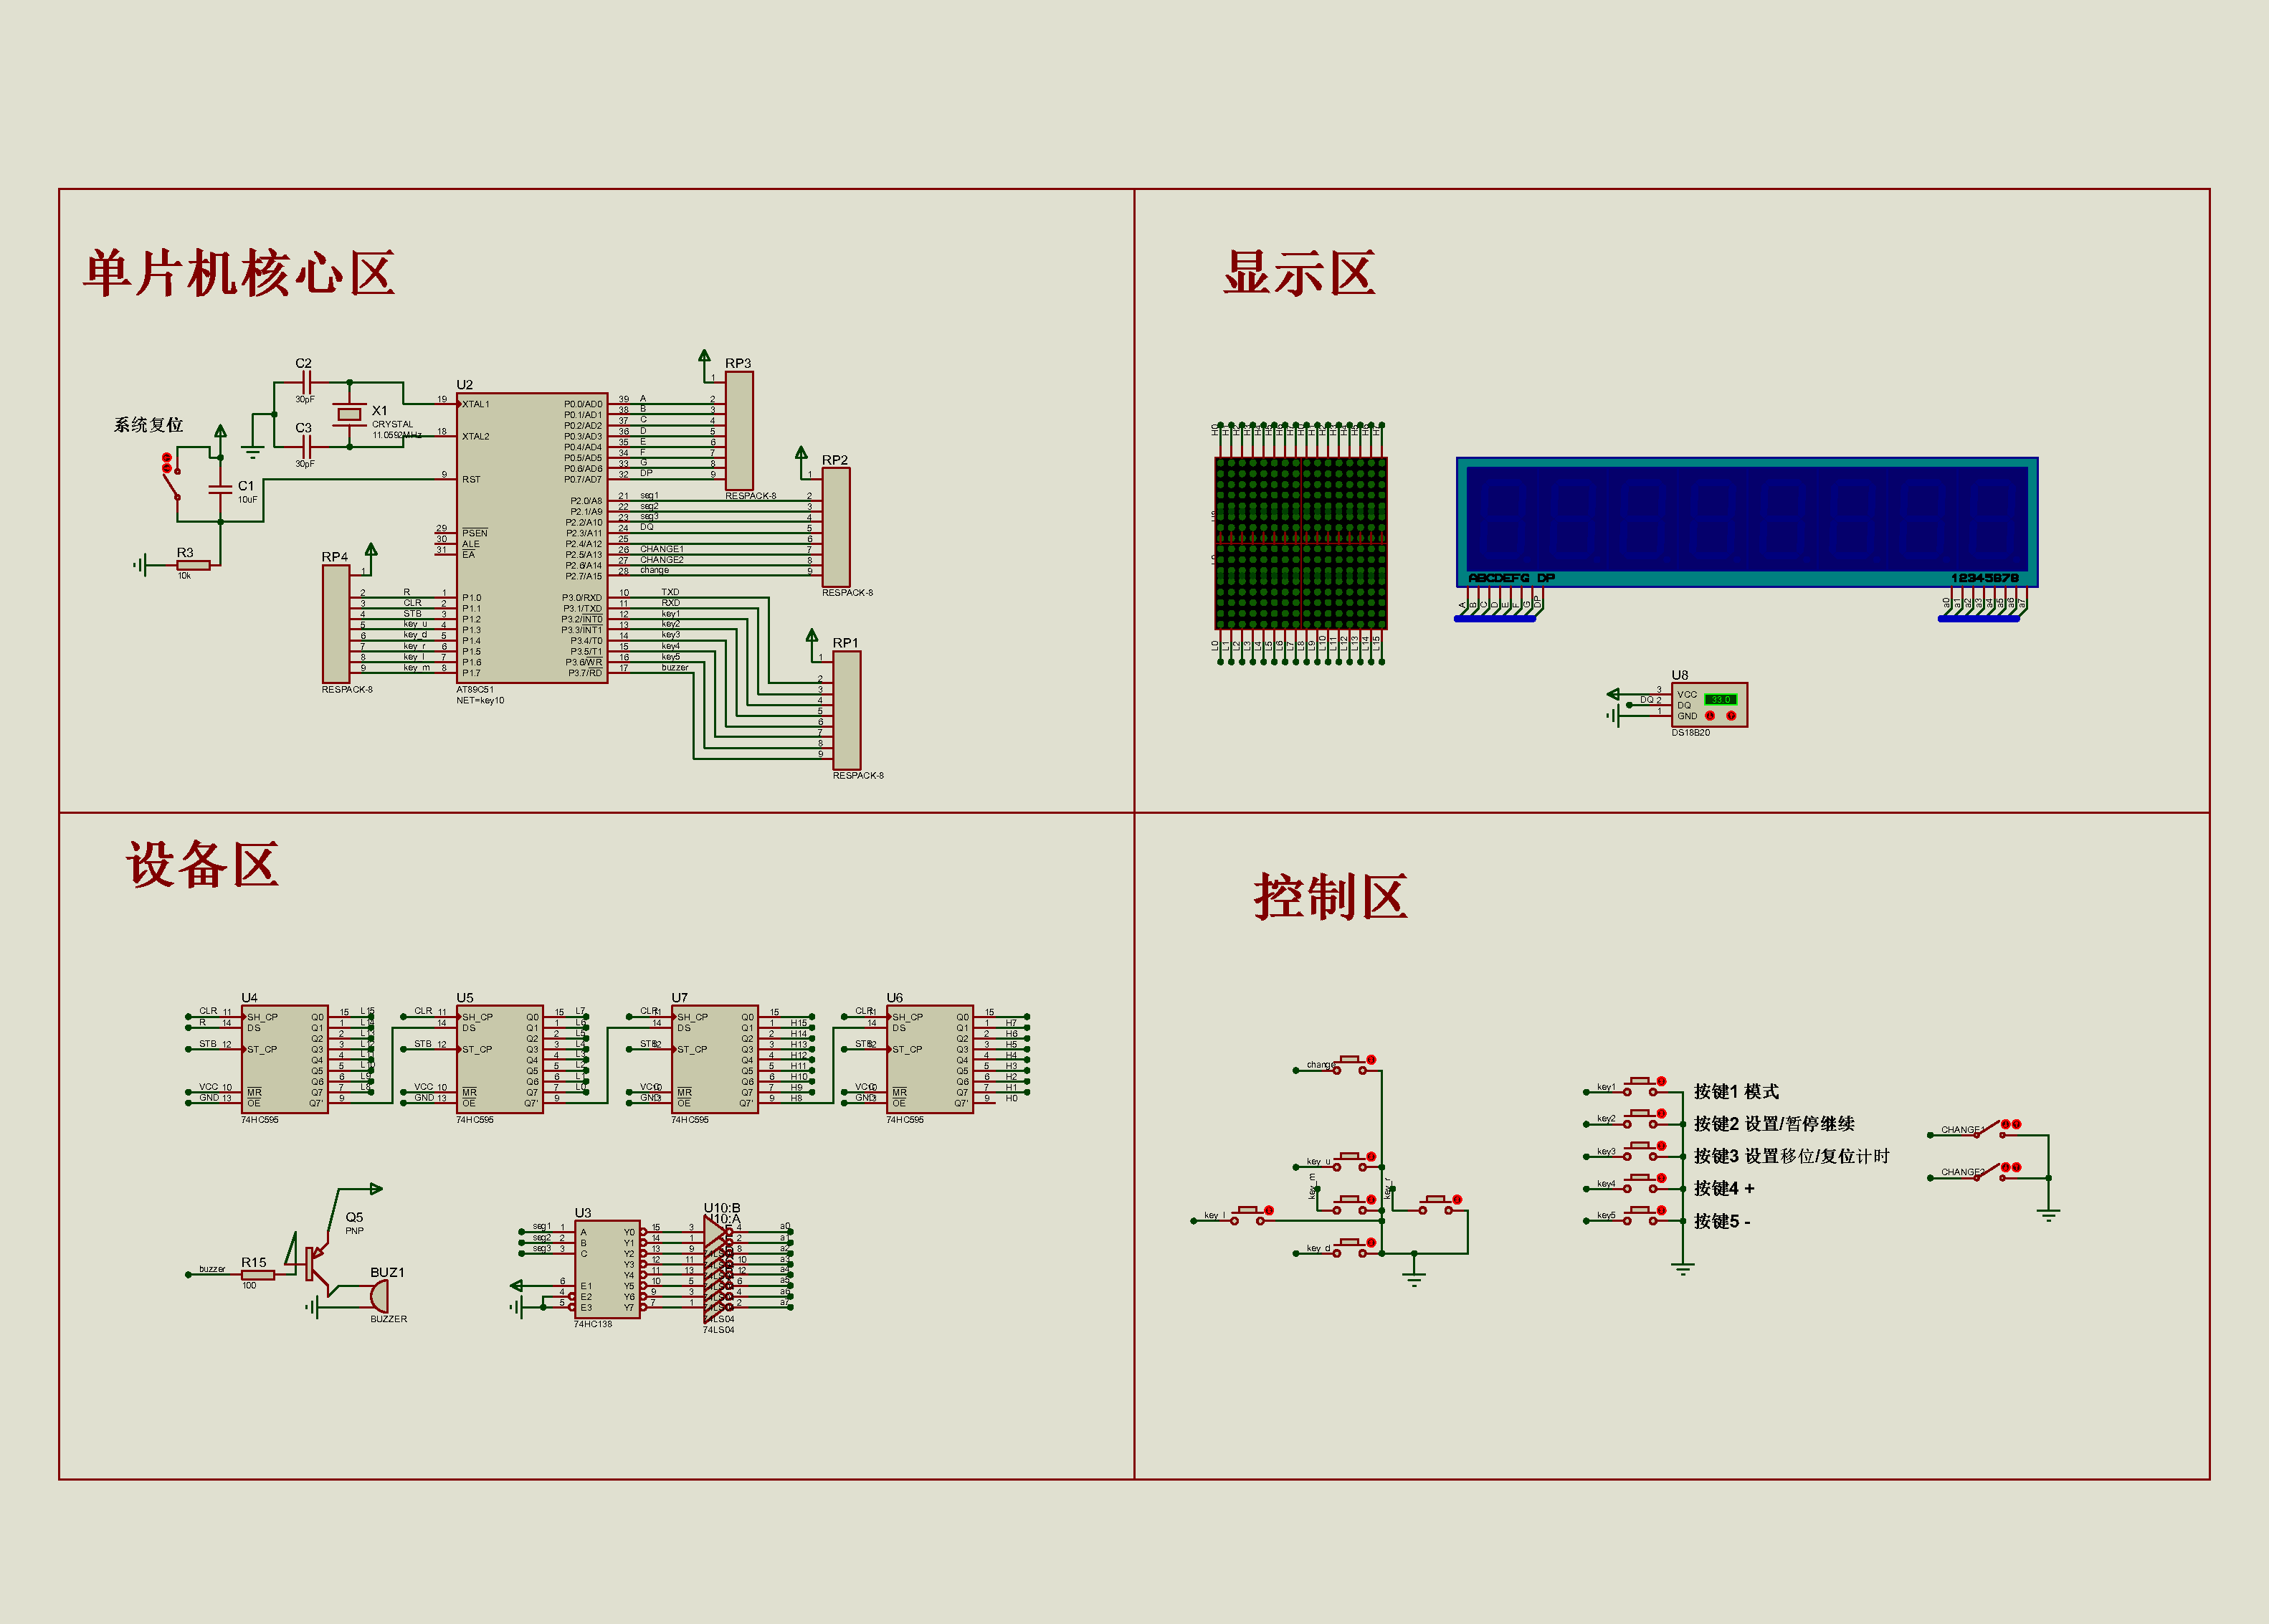
\includegraphics[scale=0.2]{Fig/项目仿真图.pdf}
	\caption{本项目电路原理仿真图}\label{Fig.33}
	\end{figure}

	
	\subsubsection{单片机核心区}
	本项目核心区采用AT89C51芯片,是项目的核心区域。

	
	\subsubsection{设备区}
	设备区由串转并模块和38译码器以及蜂鸣器组成。
	
	\subsubsection{显示区}

	\begin{figure}[htbp]
	\centering
	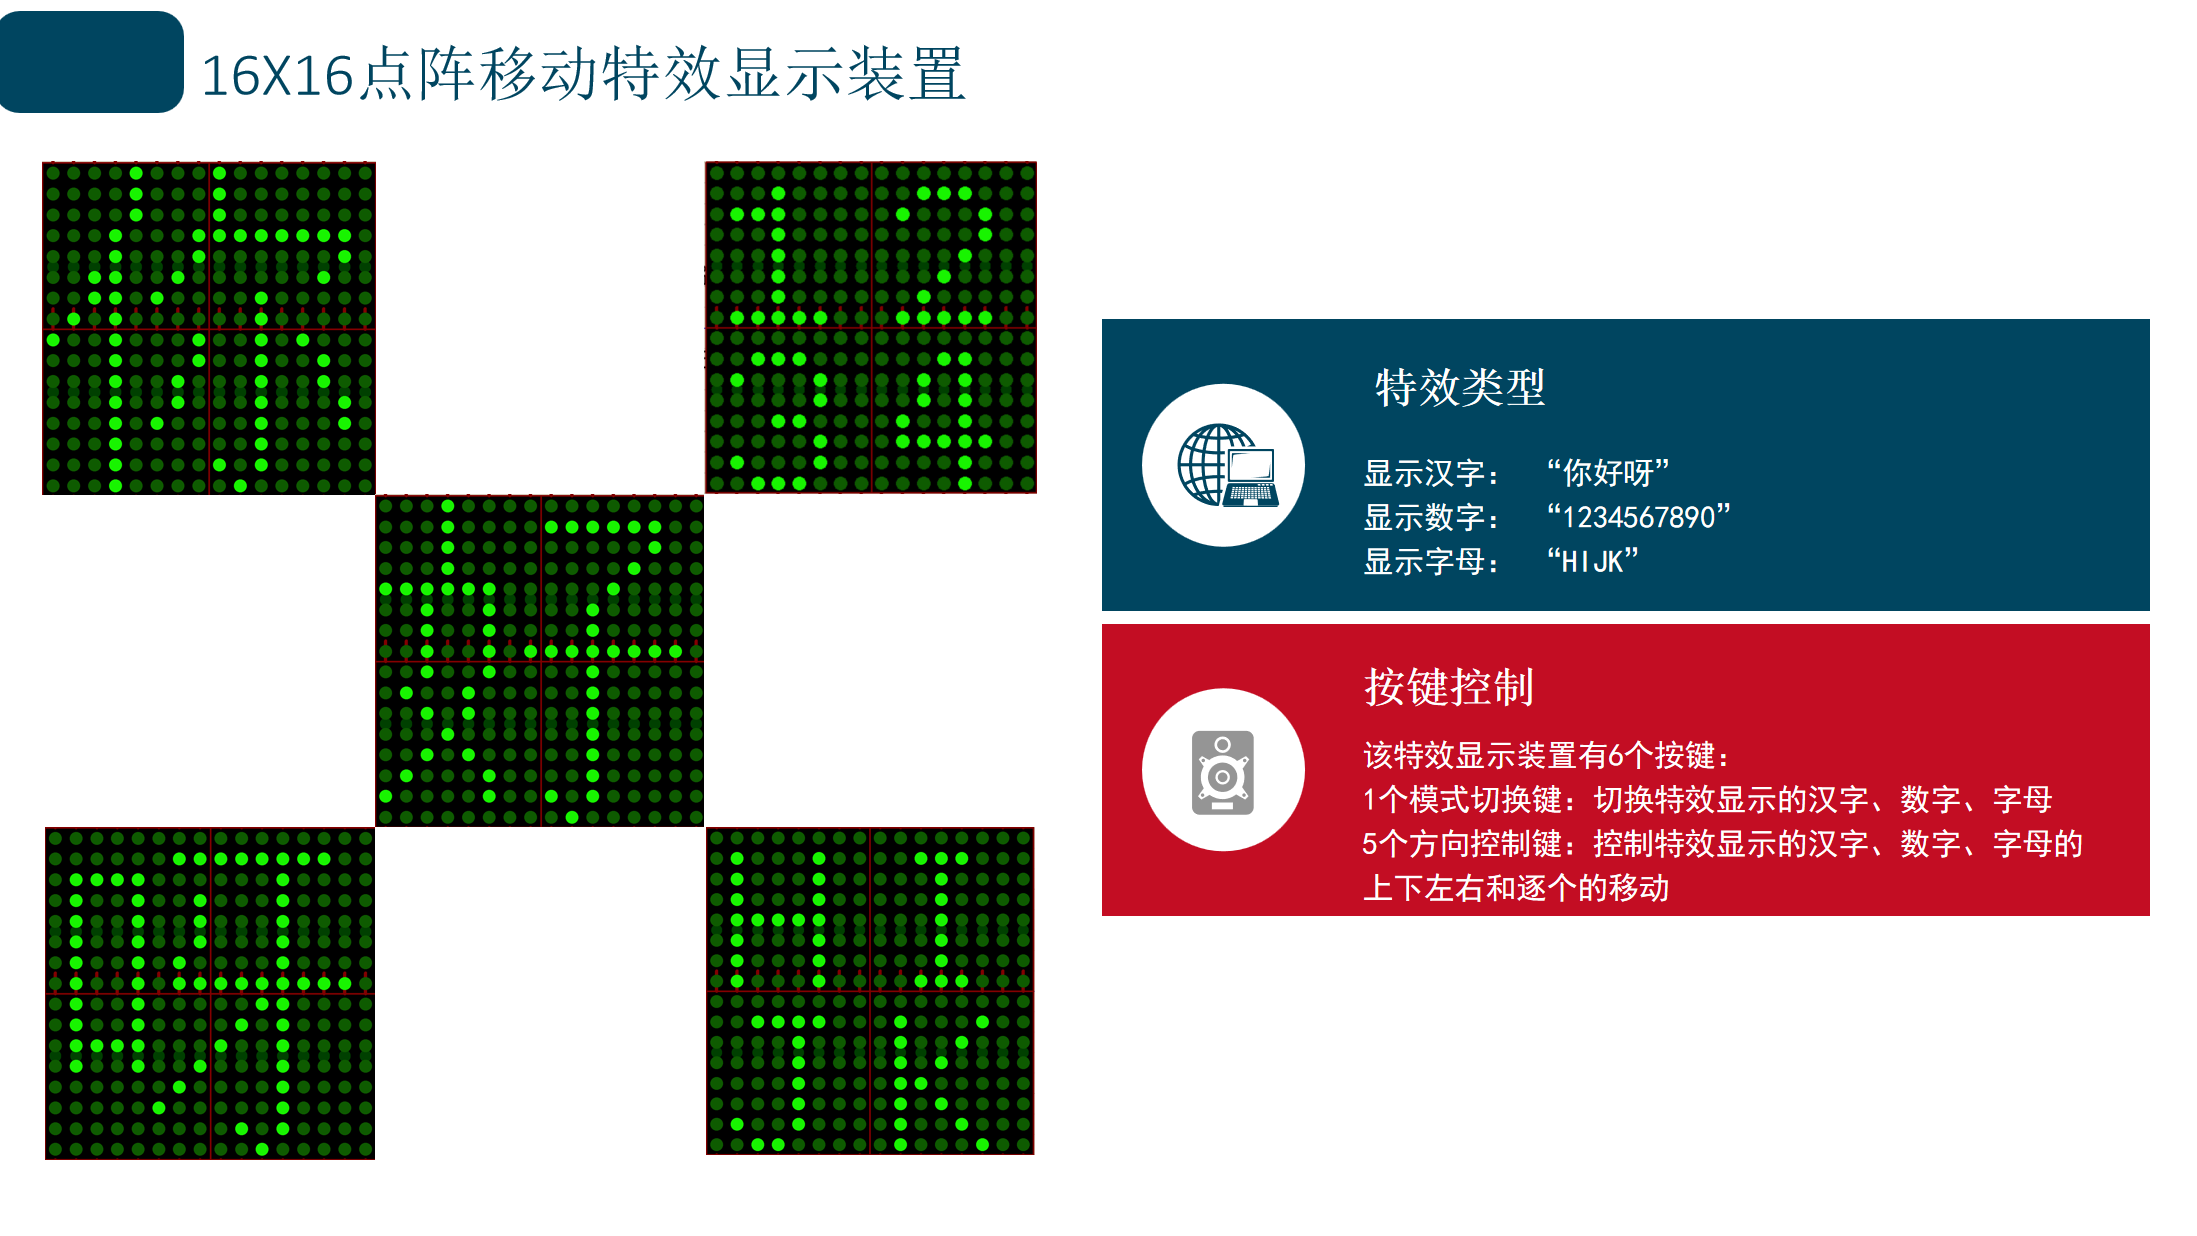
\includegraphics[scale=0.2]{Fig/显示区1.png}
	\caption{16X16点阵移动特效显示装置}\label{Fig.34}
	\end{figure}

	\begin{figure}[htbp]
	\centering
	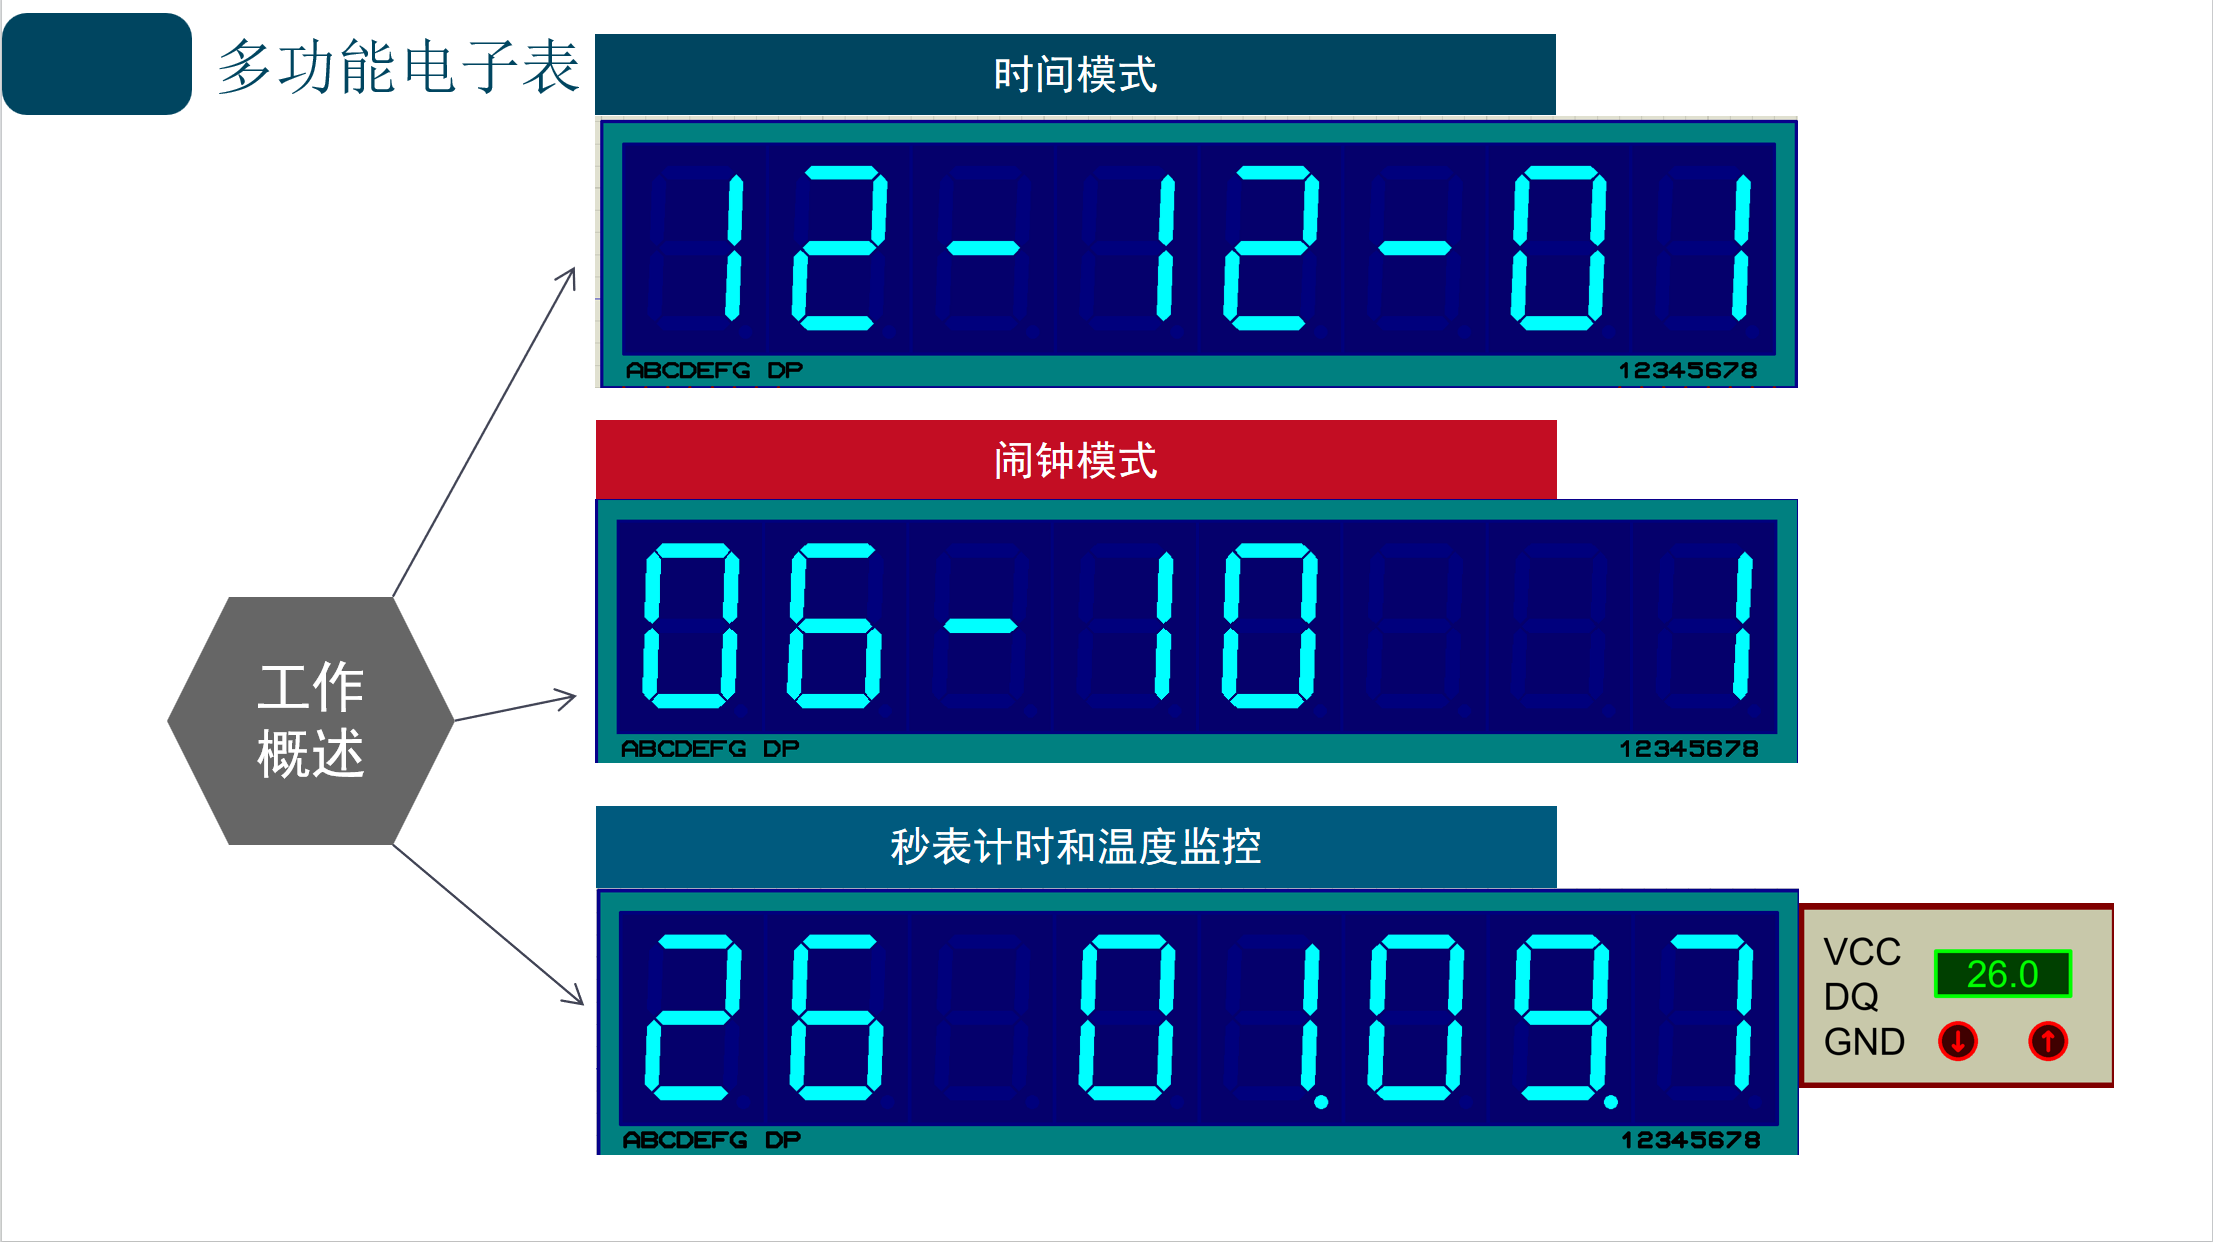
\includegraphics[scale=0.2]{Fig/显示区2.png}
	\caption{多功能电子表}\label{Fig.35}
	\end{figure}


	
	\subsubsection{控制区}
	我们通过使用多个BUTTON和SWITCH开关组合来控制整个项目功能的实现,具体如图1、图2和图3所示
	
	%\ref{Fig.11}、\ref{Fig.12}和\ref{Fig.13}所示为控制区仿真图
	
	\begin{figure}[htbp]
		\centering
		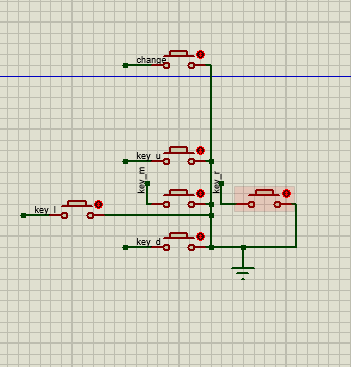
\includegraphics[scale=0.4]{Fig/控制区一.png}
		\caption{控制16x16点阵控制特效显示装置}\label{Fig.36}
	\end{figure}
	
	动态扫描点阵,利用人眼视觉暂留实现点阵移动特效。
	
	该特效显示装置有6个按键:
	
	1个模式切换键:切换特效显示的汉字、数字、字母
	5个方向控制键:控制特效显示的汉字、数字、字母的上下左右和逐个的移动
	
	特效类型:
	
	显示汉字: “你好呀”
	
	显示数字: “1234567890”
	
	显示字母: “HIJK”
	
	注:
	利用了74HC595芯片的io拓展功能(串转并模块),让一个74HC595能控制8个引脚,级联使4个74HC595控制32个引脚,刚好是横总向各16个。设计有六个按键来控制整体的显示特效切换。
	
	\begin{figure}[htbp]
		\centering
		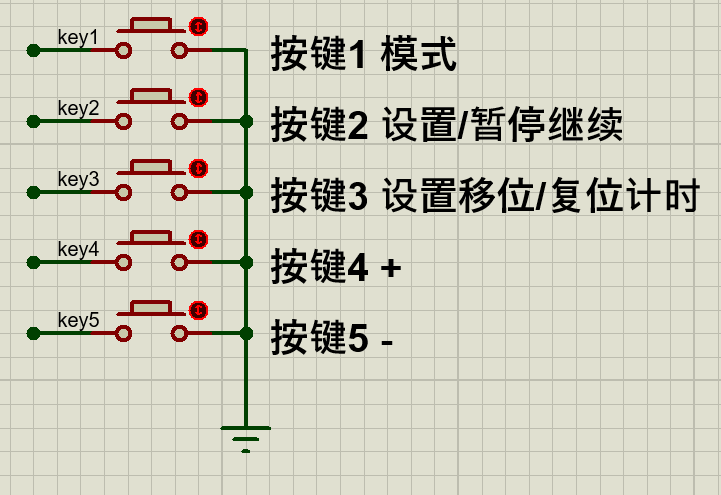
\includegraphics[scale=0.3]{Fig/控制区二.png}
		\caption{控制多功能电子表}\label{Fig.37}
	\end{figure}
	
	多功能电子表使用51单片机对8位数码管动态扫描显示,实现时间闹钟等量的显示。通过单线协议与ds18b20通信可获得此时的温度值。
	
	该表有5个按键
	
	按键1:模式键
	
	按键2:设置/暂停/继续
	
	按键3:设置移位/复位计时
	
	按键4:+
	
	按键5:-
	
	3个模式:时间模式、闹钟模式、温度及秒表计时模式
	
	时间模式:实时显示时间(时分秒)
	
	闹钟模式:设置闹钟时间,开启/关闭闹钟,利用蜂鸣器闹铃
	
	温度及秒表计时模式:读取并显示实时温度,秒表计时
	
	注:
	按键1是模式,来控制显示的实时时间、闹钟时间、温度及秒表计时功能。在任意模式下都能按设置功能(按键2)进行设置,再按一次是确认。按键4和5是增加减少的按键。按键3是移位的按键,在设置时间、闹钟时候切换位数设置数值用的。其中闹钟可以设置是否开启。在秒表计时模式下,可以直接读取到温度值,按键2控制开始和暂停,按键3可以控制复位秒表计时数值。
	
	\begin{figure}[htbp]
		\centering
		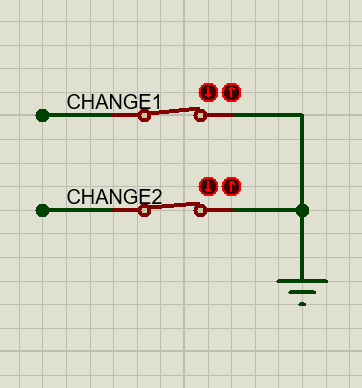
\includegraphics[scale=0.4]{Fig/控制区三.png}
		\caption{控制项目的开和关}\label{Fig.38}
	\end{figure}
	CHANGE1是控制16x16点阵特效显示器的开关
	
	CHANGE2是控制多功能电子表的开关
	
	当开关连通即为开启,开关断开即为关闭。
	
	
	\vspace{1cm}
	
	\subsection{代码实现}                       %4.2
	本项目由4个C语言主源文件和5个头文件组成.
	
	有主函数源文件main.c、主要功能函数源文件function.c、函数温度监控实现源文件temperature.c和延时函数源文件delay.c以及51单片机库函数头文件reg51.h、主要头文件header.h、延时函数头文件delay.h、串口通信头文件uart.h、温度监控头文件temperature.h。
	
	\begin{figure}[htbp]
		\centering
		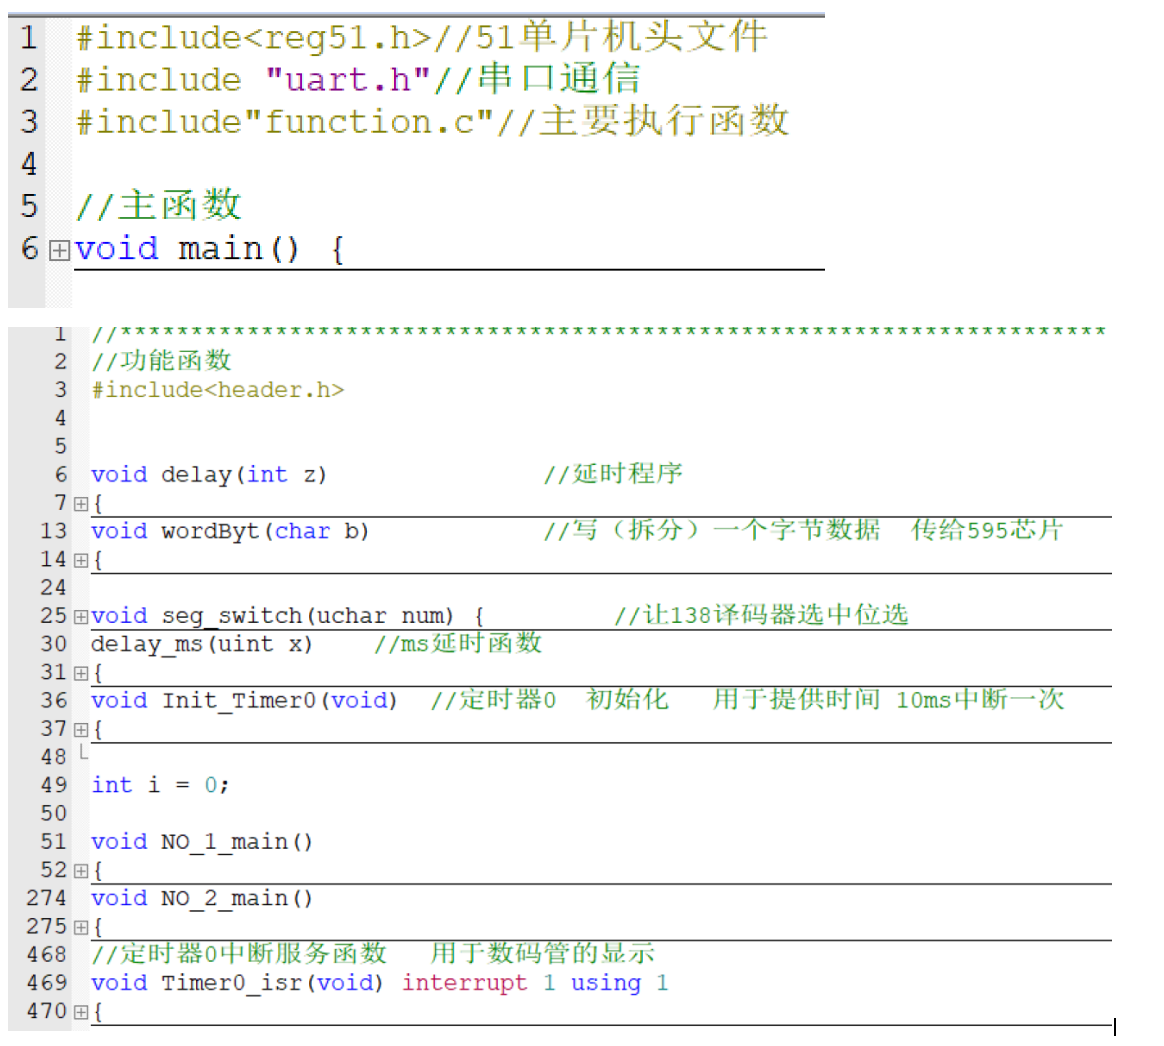
\includegraphics[scale=0.5]{Fig/代码.png}
		\caption{主要代码}\label{Fig.41}
	\end{figure}
	
	\begin{figure}[htbp]
		\centering
		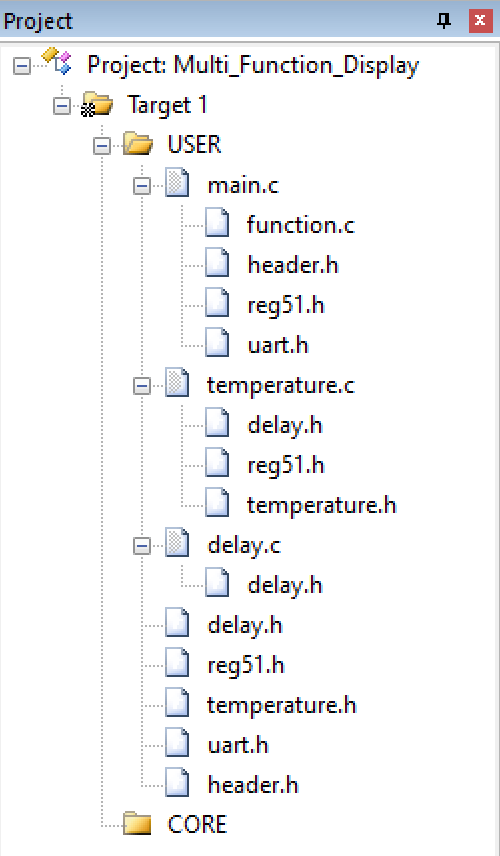
\includegraphics[scale=0.7]{Fig/代码集.png}
		\caption{代码集}\label{Fig.40}
	\end{figure}
	
	
	
\section{实训总结}					 		%五
	\subsection{尹仁标}
	在本次实训中,我们团队成功设计并实现了一款具备多种功能的显示器,这不仅是一项技术实践,更是一次深刻的学习体验。通过将课堂上学到的理论知识与实际操作相结合,我们亲手将零散的电子元件组装成了一个功能完备的系统。在这个过程中,我们深入理解了各个元件的工作机制,掌握了单片机开发的基本流程,并且真正体验到了从零开始设计项目所带来的成就感。
	
	实训期间,我们经历了从初步设计到最终实现的全过程,期间充满了挑战和乐趣。我们在实践中发现问题,解决问题,每一个小小的突破都让我们的编程能力和实验设计技巧更进一步。这段经历让我们深刻认识到,理论知识是基础,但将其应用到实践中才能真正发挥其价值。
	
	团队合作在这次实训中发挥了至关重要的作用。我们相互支持,共同面对困难,一起攻克了众多技术难题。这次经历让我深刻体会到团队协作的力量,以及每个成员在团队中的重要性。我们相互鼓励,共同进步,这种团队精神将是我们今后学习和工作中的宝贵财富。
	
	在实训过程中,我们不仅学到了知识和技能,更重要的是学会了如何学习和工作的方法。正如我们的实训老师杨翌虢所强调的:“让优秀成为习惯。”这句话深深影响了我们,让我们意识到追求卓越不仅仅是一种目标,更是一种态度,一种习惯。我相信,通过这次实训,我们不仅提升了自己的技术水平,更为未来的发展奠定了坚实的基础。
	
	总结这次实训,我们收获的不仅是技术知识,更是一种面对问题的勇气,一种解决问题的能力,一种团队合作的精神。这些宝贵的经验和技能,将伴随我们在未来的学习和工作中,不断追求卓越,不断超越自我。
	\
	\subsection{华文超}
	在本次实训中,我们团队完成了一个具有里程碑意义的项目——多功能显示器的设计和实现。这不仅是一项技术任务,更是一次全面而深入的学习旅程。通过这次实训,我们不仅将书本上的理论知识和实训老师教授的专业技能付诸实践,更在动手操作中深刻理解了各个电子元件的工作原理和单片机开发实验的基本步骤。
	
	我们从最基本的电路设计开始,一步步地将概念转化为现实。在这个过程中,我们体会到了设计一个项目所带来的无尽乐趣和挑战。每一次的电路调试,每一段代码的编写,都让我们对电子工程有了更加深刻的认识。在这段时间里,我们的实验室充满了欢声笑语,也不乏疑惑和汗水。每当遇到难题,我们都会集思广益,共同寻找解决方案,这种团队协作的精神让我们克服了一个又一个难关。
	
	在实训过程中,我们遇到了不少问题,但正是这些问题的发现和解决,极大地提升了我们的编程能力和实验设计能力。我们学会了如何分析问题,如何快速定位问题源头,以及如何高效解决问题。这些能力对我们未来的学习和工作都是极其宝贵的财富。
	
	团队合作在这次实训中发挥了至关重要的作用。我们分工明确,相互协作,每个人都在各自的岗位上发挥着重要作用。我们相互支持,共同面对困难,一起攻克了众多技术难题。这次经历让我深刻体会到团队协作的力量,以及每个成员在团队中的重要性。我们相互鼓励,共同进步,这种团队精神将是我们今后学习和工作中的宝贵财富。
	
	我们的实训老师杨翌虢老师不仅传授给我们专业知识,更教会了我们许多学习和工作的方法。他经常强调:“让优秀成为习惯。”这句话深深影响了我们,让我们意识到追求卓越不仅仅是一种目标,更是一种态度,一种习惯。我们学会了如何持续地提升自己,如何在每一个项目中追求更高的标准。
	
	总结这次实训,我们收获的不仅是技术知识和实践经验,更是一种面对问题的勇气,一种解决问题的能力,一种团队合作的精神。这些宝贵的经验和技能,将伴随我们在未来的学习和工作中,不断追求卓越,不断超越自我。我们相信,通过这次实训,我们已经为未来的学习工作打下了坚实的基础,我们有信心达到更高的高度。
	
	
\section{小组分工和组员风采}					%六


\subsection{小组分工}	
	\begin{itemize}
		\item 尹仁标:收集资料、编写代码、组装电路仿真图、编写LaTex实训报告、完善PPT、录制项目视频、参与项目答辩
		
		
		\item 华文超:整理资料、封装代码、绘制电路仿真图、编写LaTex实训报告、制作PPT、录制项目视频、参与项目答辩
		
	\end{itemize}


\subsection{组员风采}	
	\begin{figure}[htbp]
		\centering
		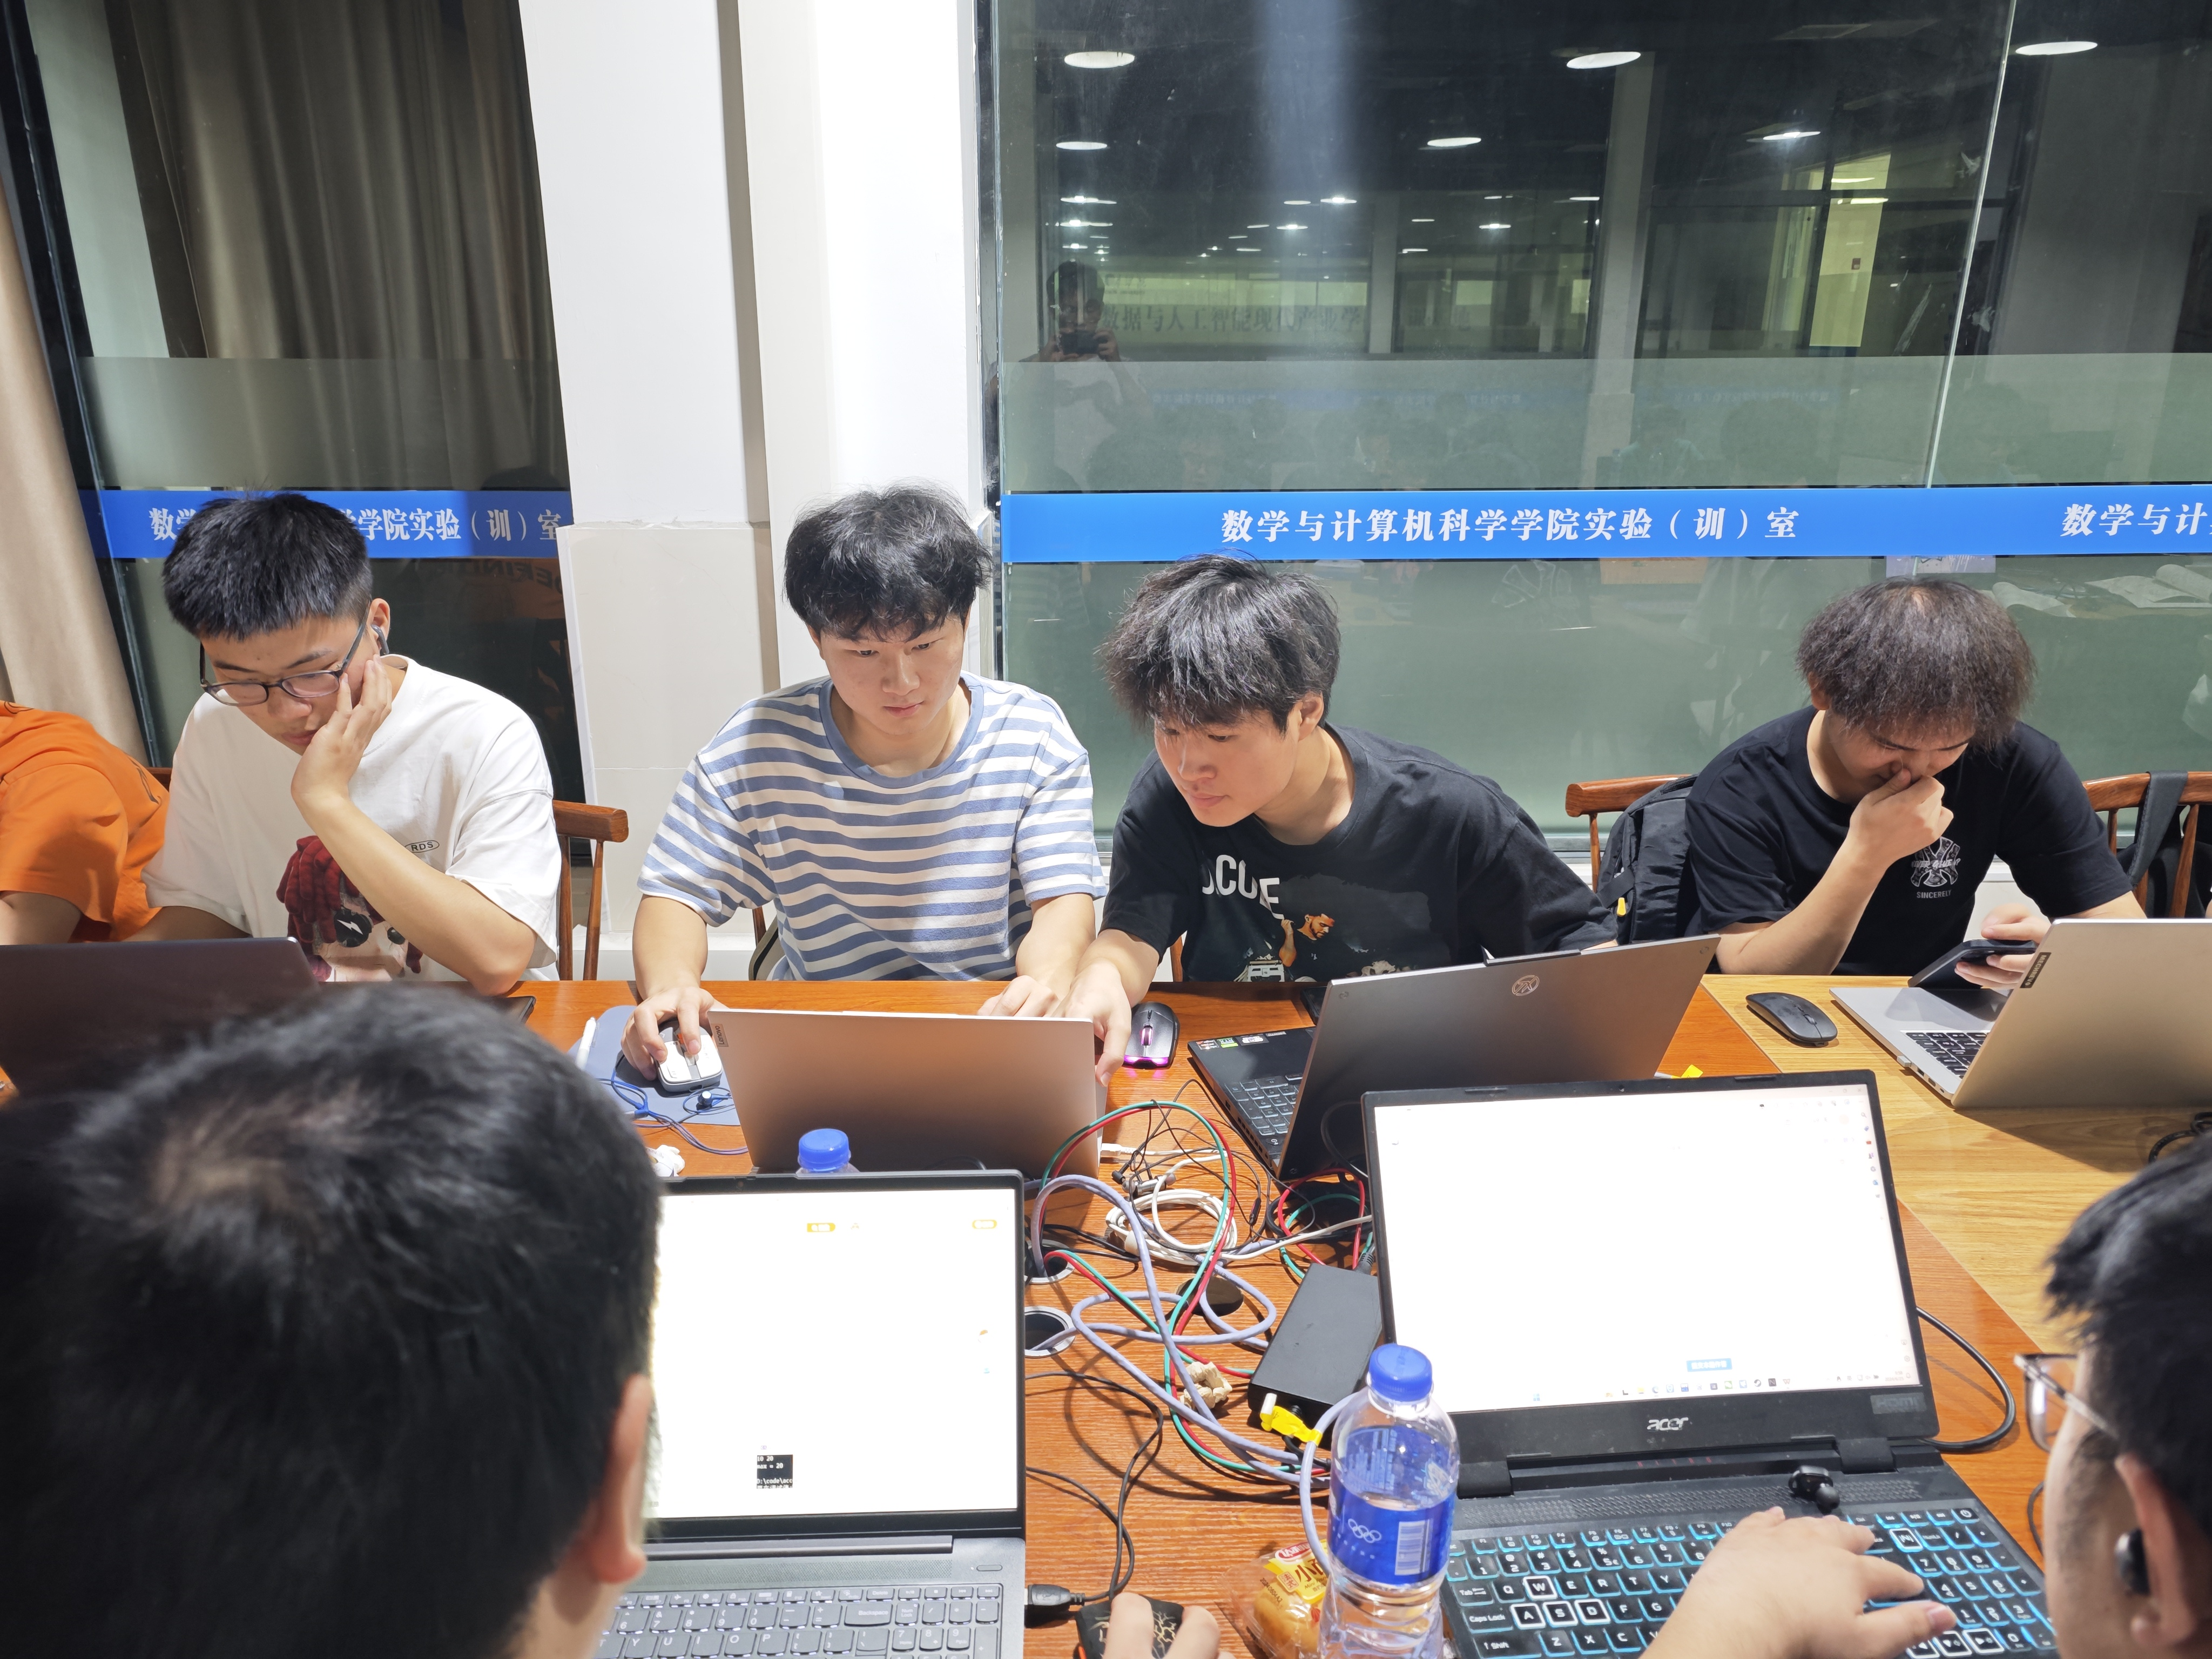
\includegraphics[scale=0.1]{Fig/1.jpg}
		\caption{实训1}\label{Fig.42}
	\end{figure}
	
	\begin{figure}[htbp]
		\centering
		
\includegraphics[scale=0.1]{Fig/2.jpg}
		\caption{实训2}\label{Fig.43}
	\end{figure}
	
	\begin{figure}[htbp]
		\centering
		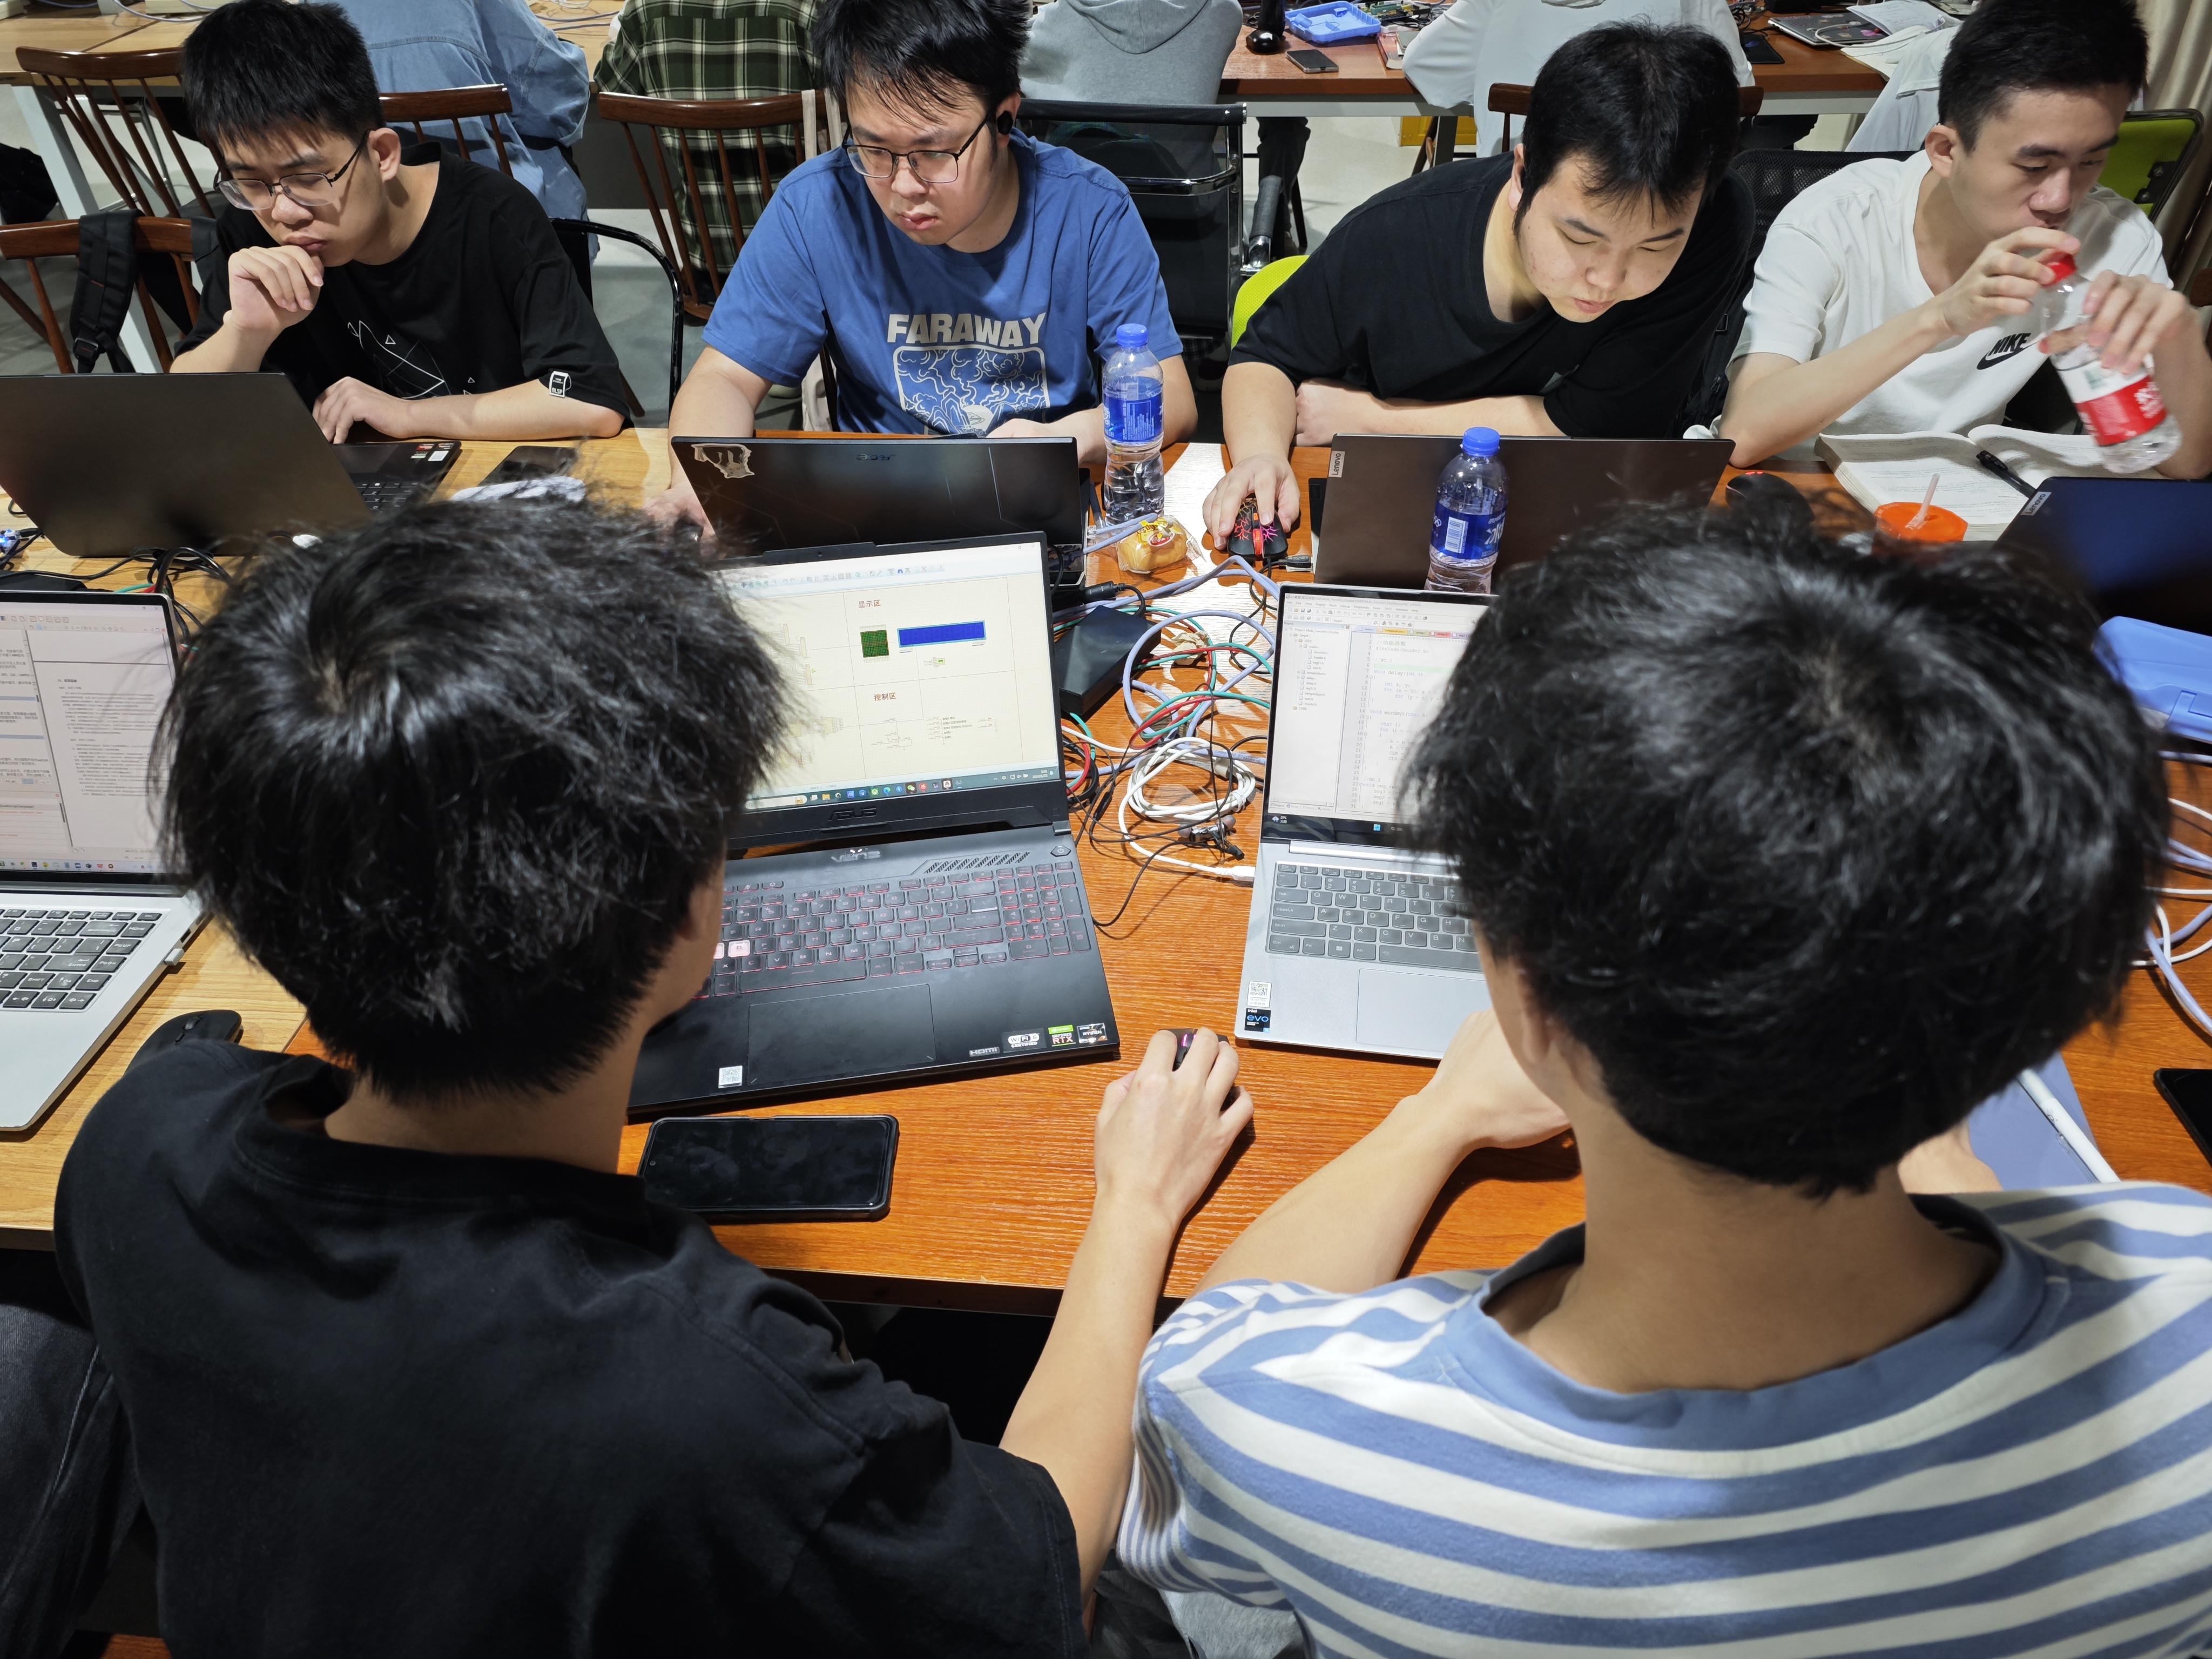
\includegraphics[scale=0.1]{Fig/3.jpg}
		\caption{实训3}\label{Fig.44}
	\end{figure}
	
	\begin{figure}[htbp]
		\centering
		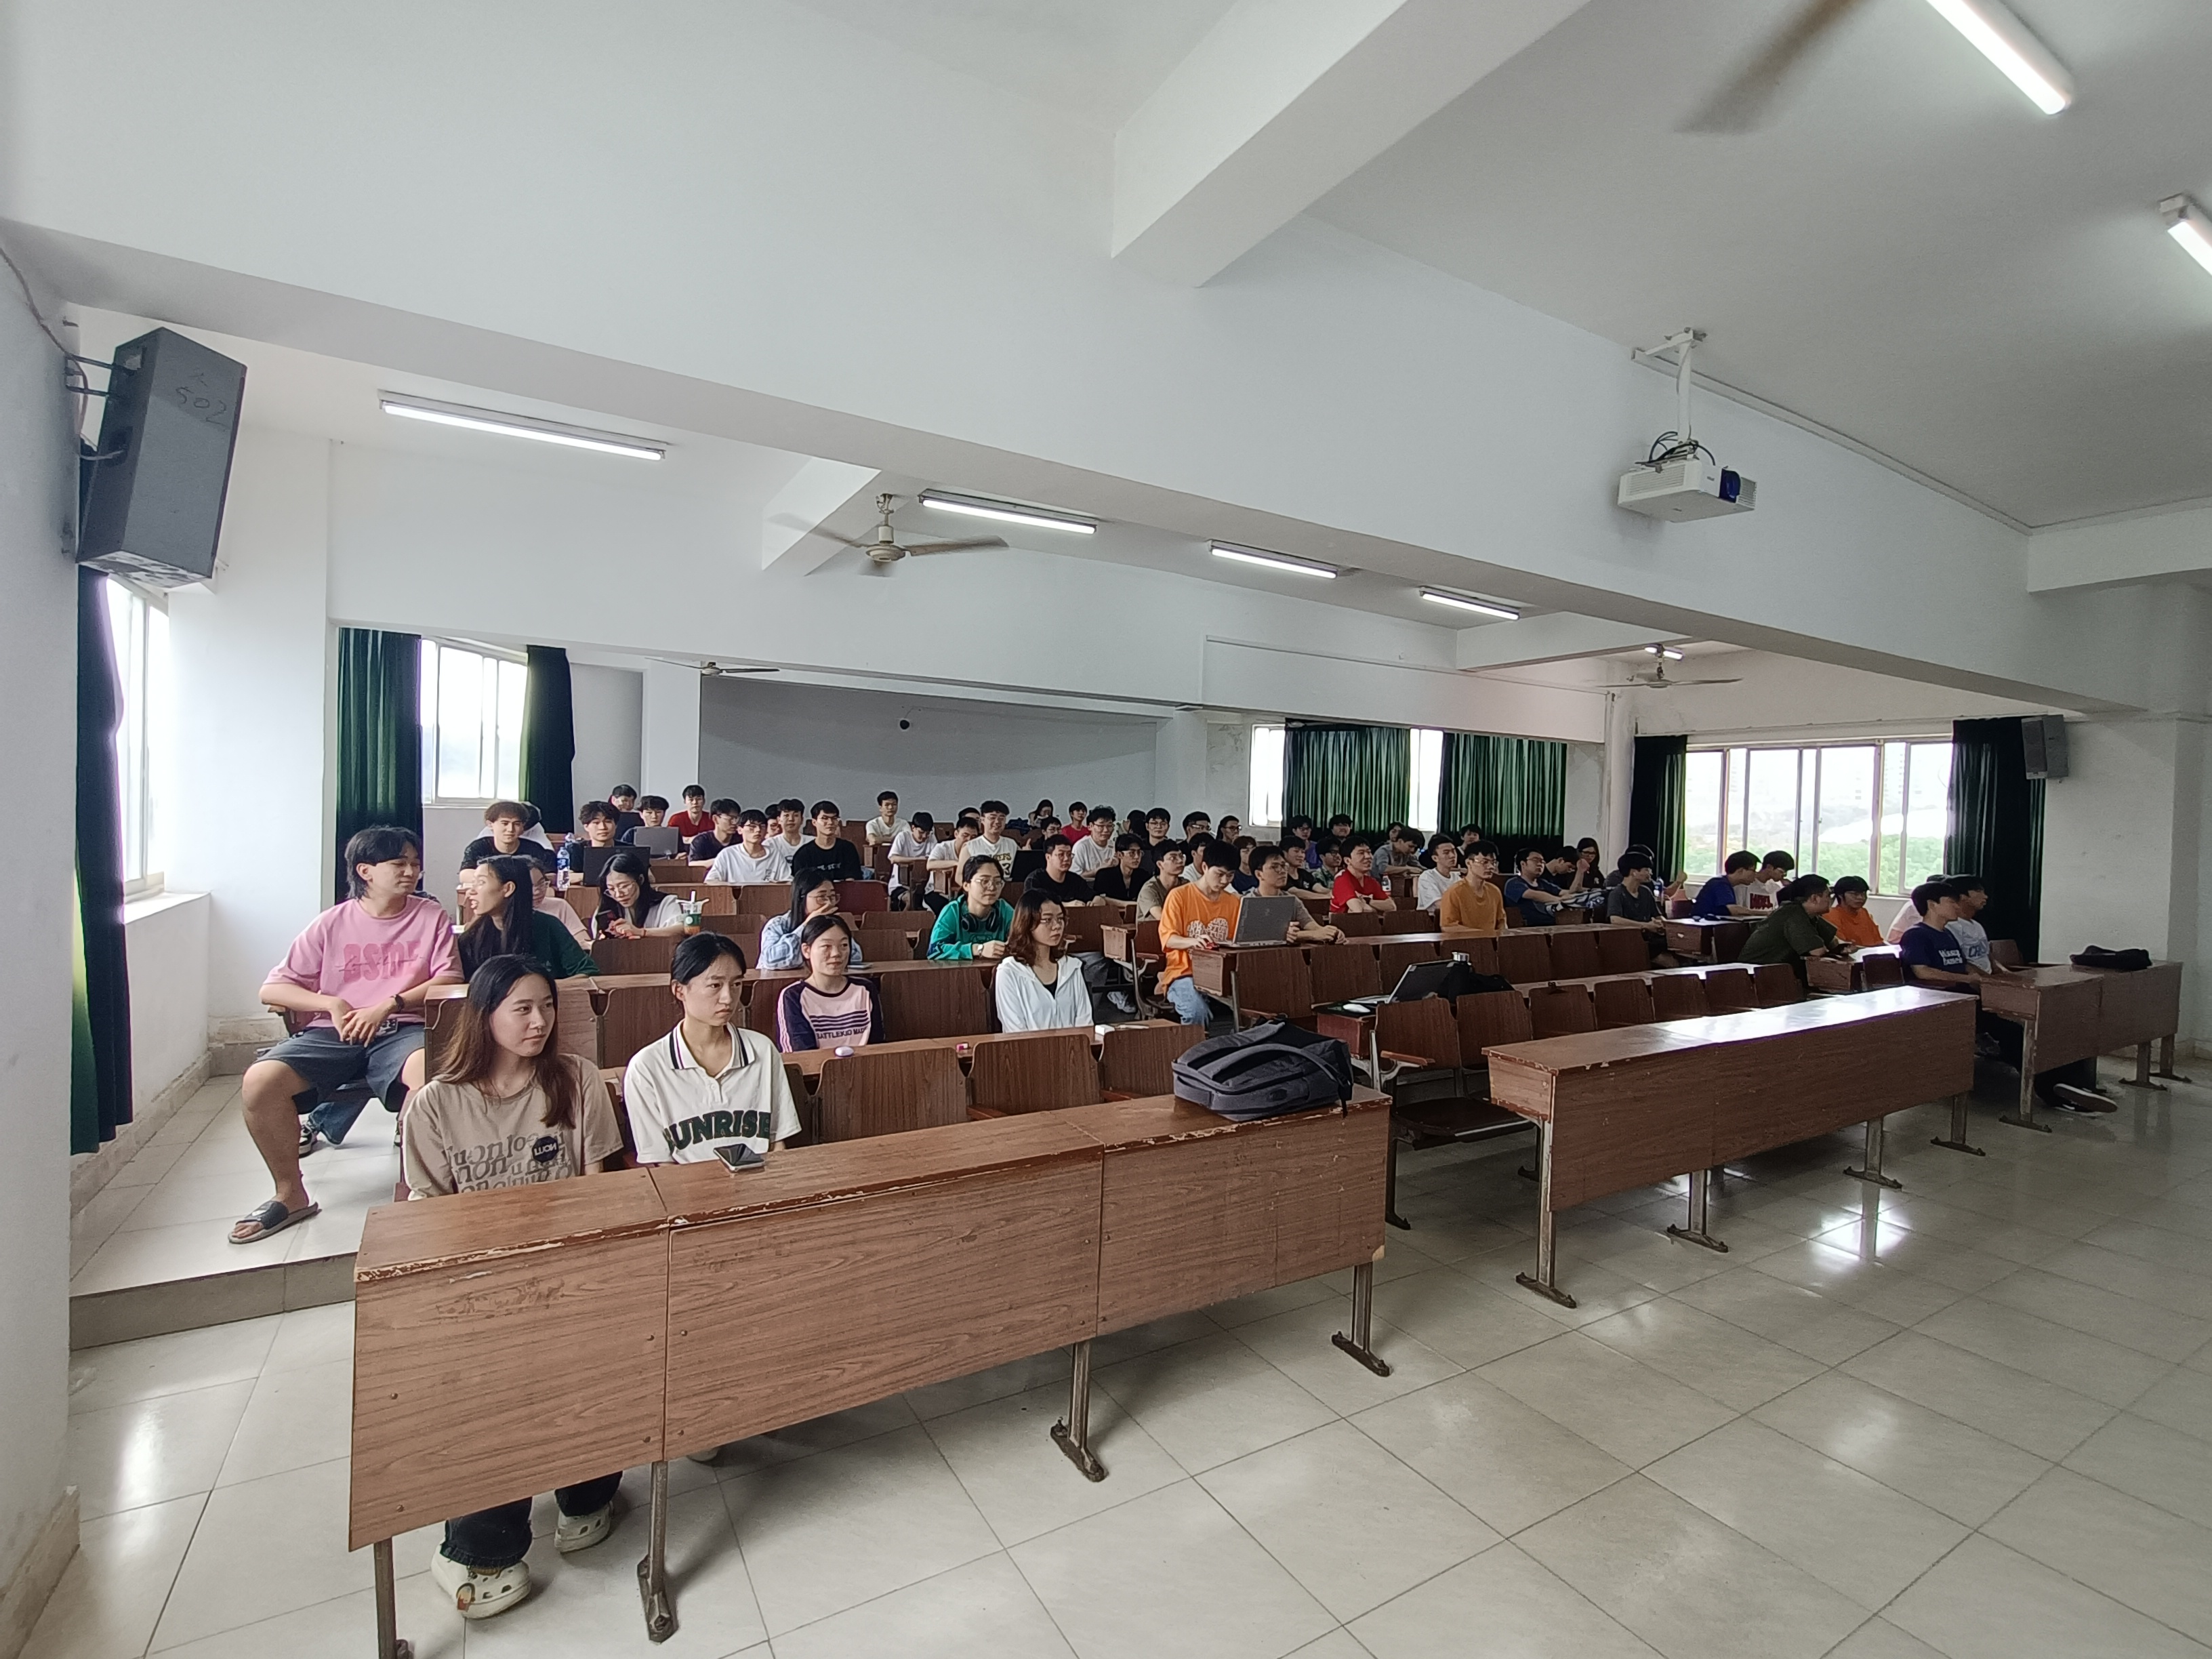
\includegraphics[scale=0.1]{Fig/合影2.jpg}
		\caption{答辩现场}\label{Fig.45}
	\end{figure}
	
	\begin{figure}[htbp]
		\centering
		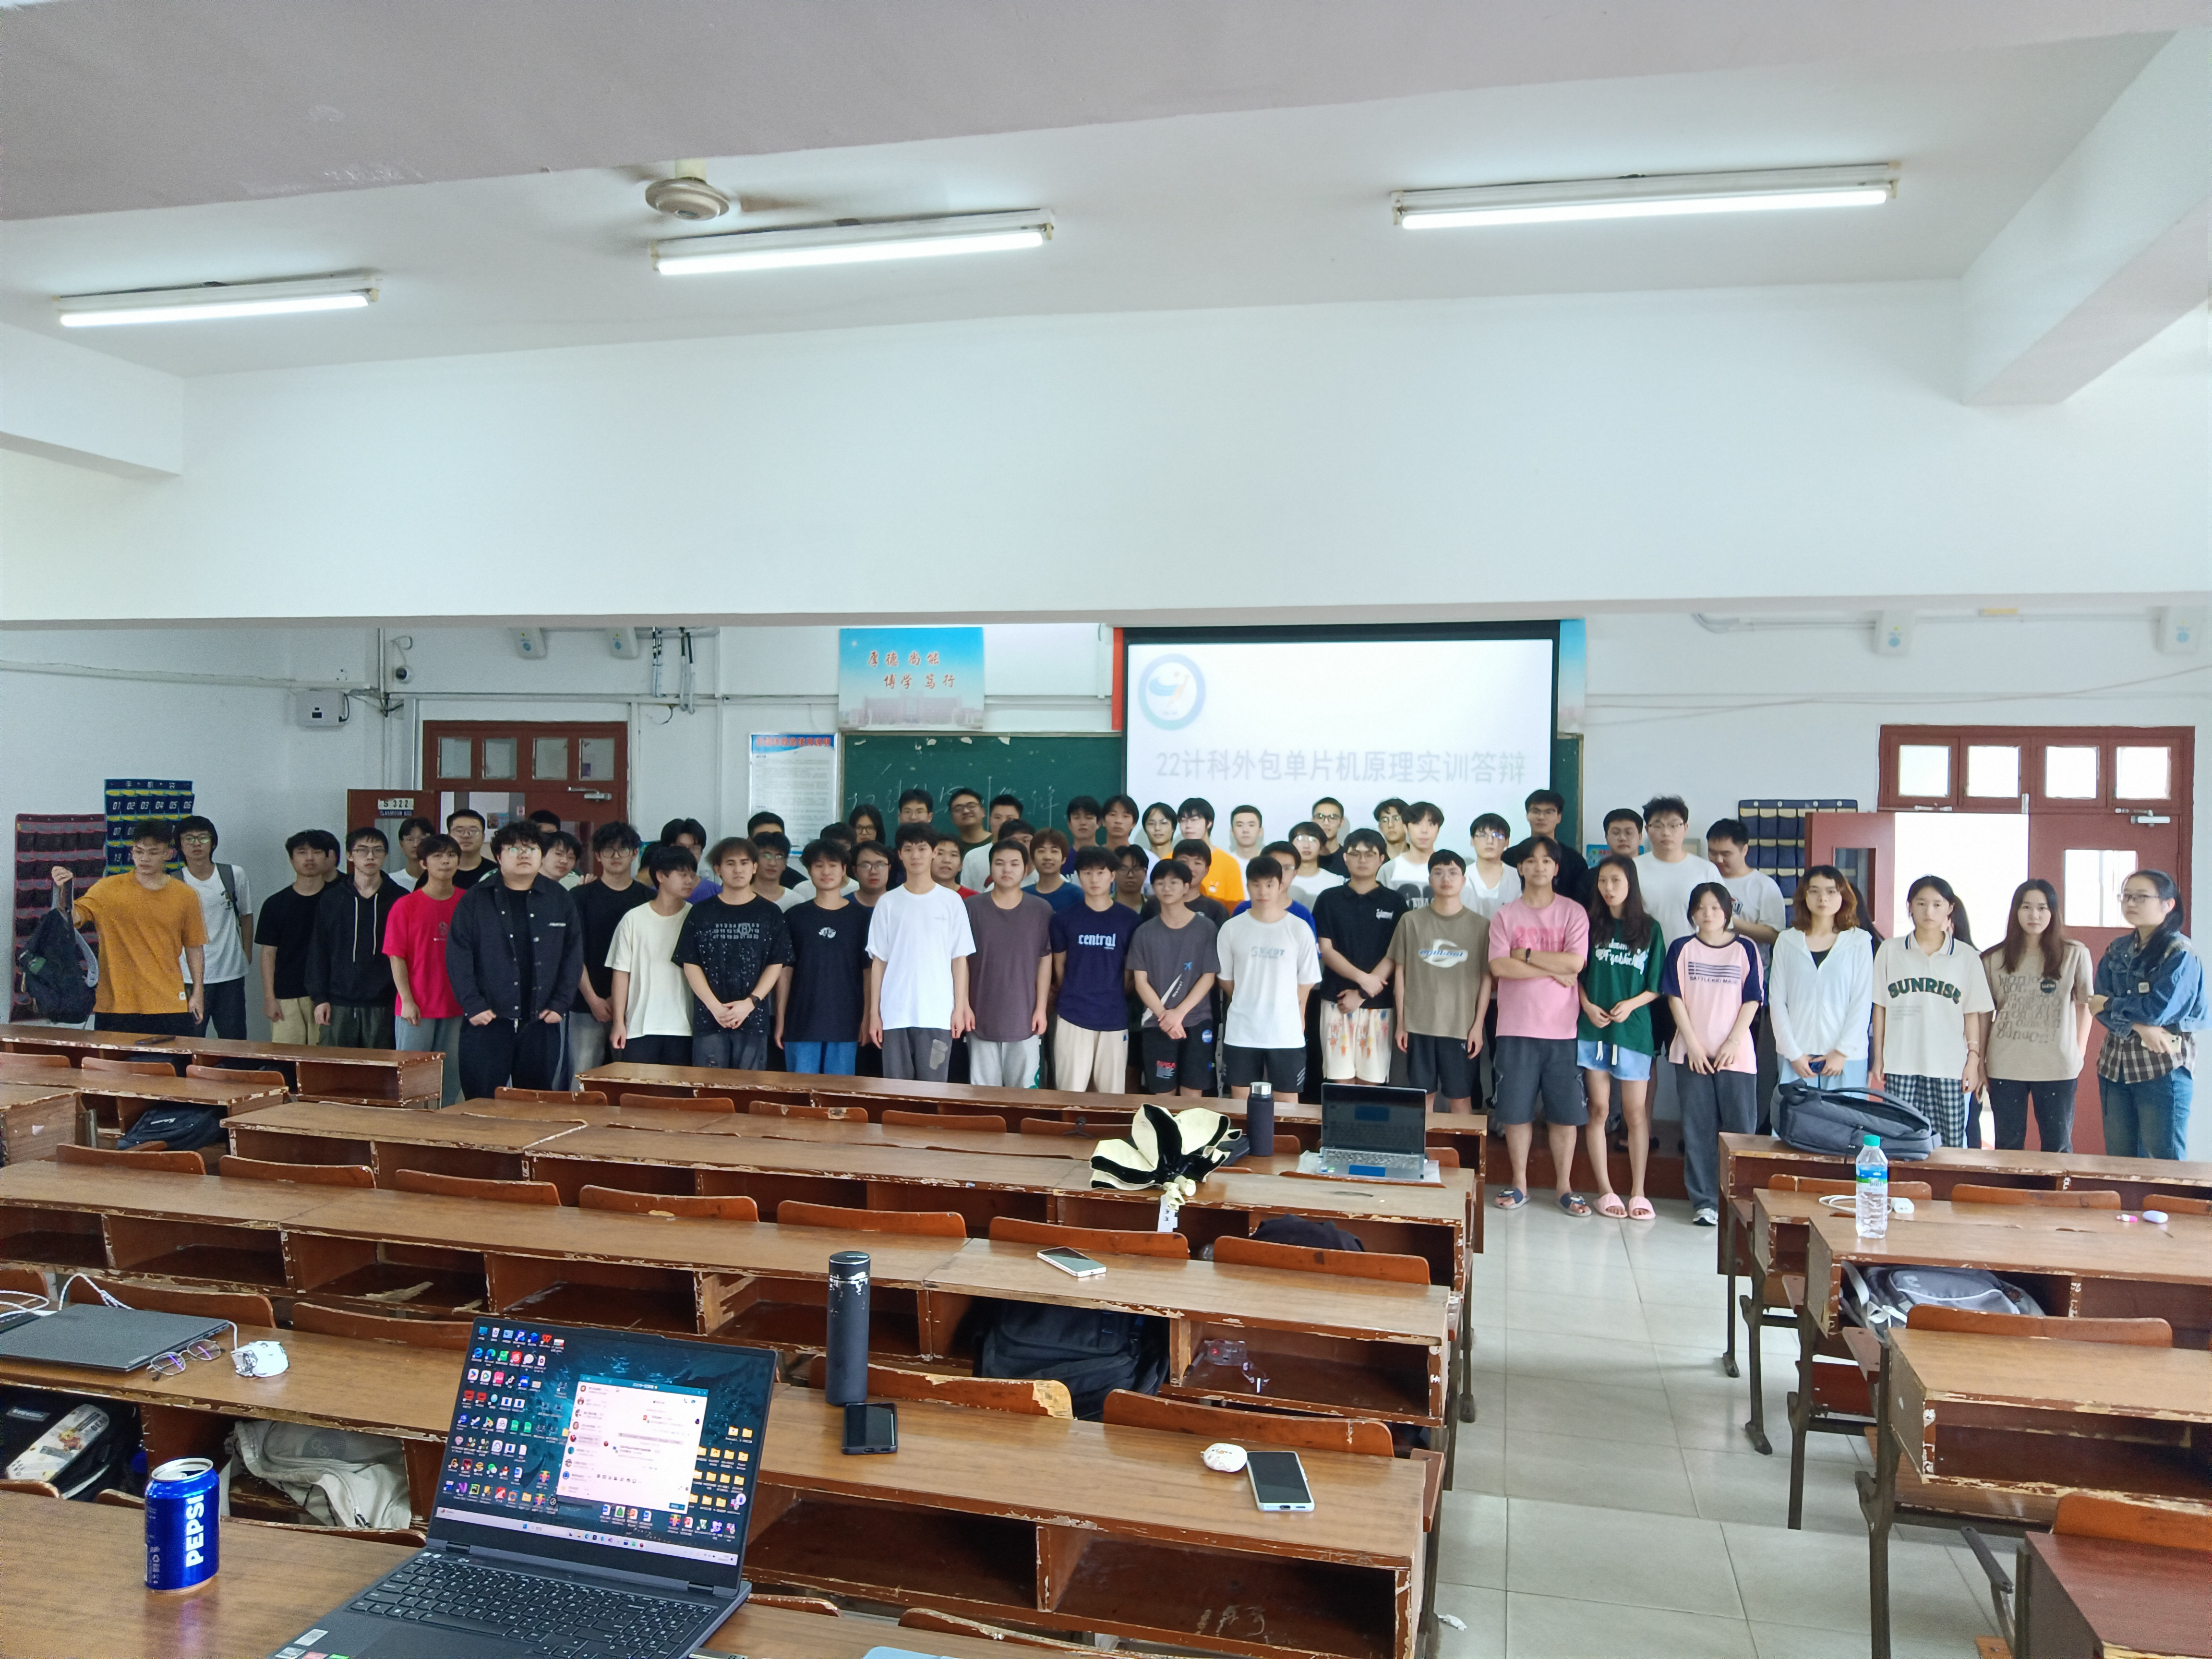
\includegraphics[scale=0.1]{Fig/合影1.jpg}
		\caption{合影}\label{Fig.46}
	\end{figure}


\section{展望}					 		  %七
在为期两周的实训期间,我们团队首次涉足单片机项目开发领域,这是一段充满挑战与发现的旅程。虽然时间紧迫,但我们的项目已经取得了初步成果,这仅仅是一个开始。我们认识到,随着技术的不断进步和市场需求的不断变化,我们的多功能显示器项目还有许多潜在的改进空间和功能待开发。

目前,我们的项目虽然已经能够实现基本的显示功能,但我们知道,要使产品更具竞争力,就必须不断优化和升级。我们计划在未来的工作中,进一步扩展显示器的功能性,比如增加触摸屏交互、无线连接能力以及更加智能的环境适应性。我们希望能够通过集成更先进的传感器和算法,使显示器能够实时响应环境变化,并提供更加个性化的用户体验。

展望未来,我们团队将持续致力于项目的完善和创新。我们相信,通过团队成员的共同努力,我们的多功能显示器将不断进步,最终实现更加全面的功能,并适用于更广泛的应用场景。我们计划引入更多的智能化元素,比如通过机器学习算法优化显示效果,或者通过大数据分析预测用户需求,从而提供更加精准和贴心的服务。

我们坚信,凭借团队的不懈努力和创新精神,我们的产品将能够满足更广泛的应用场景需求。从工业自动化到智能家居,从医疗监护到环境监测,我们的显示器都将发挥重要作用。我们期望它不仅能提供基础的显示服务,更能成为用户生活中不可或缺的智能伙伴。

为了实现这些目标,我们将继续学习和研究最新的技术趋势,不断吸收新知识,提升团队的专业能力。我们也将加强与行业内的其他专业人士和团队的交流合作,共同推动项目的发展。我们相信,通过持续的学习和合作,我们能够不断突破技术瓶颈,创造出真正具有创新性和实用性的产品。

总结这次实训,我们收获的不仅是技术知识和实践经验,更是一种面向未来的视野和决心。我们期待着在不久的将来,我们的多功能显示器能够成为市场上的一颗新星,为用户带来更加丰富和便捷的使用体验,取得更大的成功。我们相信,只要我们保持创新和努力,这一天终将到来。
	
	
\section{致谢}					     	  %八
在这段充实而宝贵的实训旅程中,我们首先要表达最深切的感激之情给我们的实训指导老师——杨翌虢老师。在项目的每一个阶段,杨老师都以他渊博的知识和无私的奉献精神,为我们提供了精心的指导和支持。他不仅在技术层面上给予我们专业的编程和实训知识,更在精神层面上激励我们,教会我们如何面对挑战,如何在压力之下保持冷静和创新思维。杨老师的教诲和榜样,对我们的学习生涯和个人成长都有着不可磨灭的影响。

我们还要向我们的团队致以崇高的敬意。在紧张而充满挑战的十天里,我们共同经历了无数的试炼和考验。每一位团队成员都展现出了难以置信的坚韧和智慧,我们相互扶持,共同进退。在遇到难题时,我们没有选择逃避,而是选择了勇敢面对,集思广益,寻找解决方案。这种团队精神不仅仅帮助我们克服了一个又一个障碍,更深化了我们之间的友谊,让我们更加紧密地团结在一起。

此外,我们对学校和数计学院的支持与帮助表示衷心的感谢。正是由于校领导和院领导的远见卓识,我们才得以拥有这样一个展示自我、挑战自我的平台。学校不仅为我们提供了先进的实验设备和舒适的学习环境,更通过邀请像杨老师这样优秀的教育者,为我们打开了知识的大门,让我们在专业领域内不断探索和进步。这份机会和资源的提供,是我们能够顺利完成项目的重要保障。

我们还要感谢所有和我们一起参与本次实训的同学和朋友,是他们的帮助和鼓励,给予了我们追求成绩和成就的动力。为我们营造了浓烈的学习环境,助力了本次实训进行。

总之,这次实训项目的成功,是我们所有人共同努力的结果。我们将会珍惜这段经历,将所学到的知识和技能,以及团队协作的精神应用到未来的学习和工作中,不断追求卓越,努力成为对社会有贡献的人。再次感谢所有支持和帮助过我们的人,没有你们,就没有我们现在的成果。


	
\end{document}
